\documentclass[11pt]{beamer}
\usepackage{graphicx}
\usepackage[export]{adjustbox}  % max width/height in includegraphics
\usepackage[framemethod=TikZ]{mdframed}
\usepackage[document]{ragged2e}

\usepackage{soul}
\usepackage{xcolor}
\usepackage{ifthen}
\usepackage{fontspec}
%\usepackage{textcomp}
%\usepackage[T5,T1]{fontenc}
\usepackage{caption}


\usetheme[hideothersubsections]{Goettingen}
\usecolortheme{seahorse}
%%% \usetheme{Montpellier}
%%% \usecolortheme{dolphin}
\setbeamercovered{invisible}
\setbeamertemplate{navigation symbols}{\insertslidenavigationsymbol}
\setbeamertemplate{page number in head/foot}{}
\setbeamertemplate{blocks}[rounded][shadow=false]
% \setbeamerfont{section in sidebar}{size=\fontsize{4}{3}\selectfont}
% \setbeamerfont{subsection in sidebar}{size=\fontsize{4}{3}\selectfont}
% \setbeamerfont{subsubsection in sidebar}{size=\fontsize{4}{2}\selectfont}


% workaround for problem that causes shadows on rounded corners to not look right
\makeatletter
\def\pgfutil@insertatbegincurrentpagefrombox#1{%
  \edef\pgf@temp{\the\wd\pgfutil@abb}%
  \global\setbox\pgfutil@abb\hbox{%
    \unhbox\pgfutil@abb%
    \hskip\dimexpr2in-2\hoffset-\pgf@temp\relax% changed
    #1%
    \hskip\dimexpr-2in-2\hoffset\relax% new
  }%
}
\makeatother


\usepackage{microtype}
% \DisableLigatures[f]{encoding = *, family = *}

%% languages and fonts
% \usefonttheme{professionalfonts} % using non standard fonts for beamer
\usepackage{tgheros}
\usefonttheme{serif}
\usepackage{XCharter}

\usepackage{xeCJK}
\usepackage{textgreek}
% \usepackage{polyglossia}
% \setdefaultlanguage{english}
% \setotherlanguage{russian}
% \newfontfamily\russianfont{/System/Library/Fonts/Times.ttc}
% \let\russianfonttt\ttfamily

% \setCJKmainfont{/System/Library/Fonts/STHeiti Light.ttc}
% \setCJKmonofont{/System/Library/Fonts/PingFang.ttc}
% \setCJKsansfont{/System/Library/Fonts/PingFang.ttc}


\AtBeginSection[]{
  \begin{frame}
    \vfill
    \centering
    \begin{beamercolorbox}[sep=8pt,center,shadow=true,rounded=true]{title}
    \usebeamerfont{title}\insertsectionhead\par%
    \ifthenelse{\equal{\thisSectionName}{Bonus}}{}{
        \usebeamerfont{subtitle}\thisSectionName\par%
    }
    \end{beamercolorbox}
    \begin{center}
    \ifthenelse{\equal{\thisSectionName}{Bonus}}{
        
\includegraphics[max height = 0.3\textheight]{Images/devilsanta.jpg}
    }{}

    Please mute yourselves!
    \end{center}

    \ifthenelse{\equal{\thisSectionName}{Bonus}}
    {
        Get ready for some \emph{devilishly} hard questions!

        \vspace*{1em}
    }{}

    \vfill
  \end{frame}
}

\AtBeginSubsection[]{
  \begin{frame}
    \vfill
    \centering
    \begin{beamercolorbox}[sep=8pt,center,shadow=true,rounded=true]{title}
    \usebeamerfont{title}\insertsectionhead\par%
    \usebeamerfont{subtitle}\insertsubsectionhead\par%
    \end{beamercolorbox}
    \ifthenelse{\equal{\subsecname}{Answers}} {
        \begin{center}
        Unmute yourselves!
        \end{center}
    }
    \vfill
  \end{frame}
}
\begin{document}

\title{Welcome to Quarantine Trivia XIII -- Holiday Edition!}
\date{}

\begin{frame}
    \titlepage{}
    \begin{center}
        
\includegraphics[max width=0.9\textwidth,
            max height=0.4\textheight]{Images/triviatitleframelogo.png}
    \end{center}
\end{frame}
\begin{frame}
    This week, we started wondering if they play trivia at the North Pole, so we sent our
    crack research team to Santa's home to find out.
    \pause
    \begin{center}
        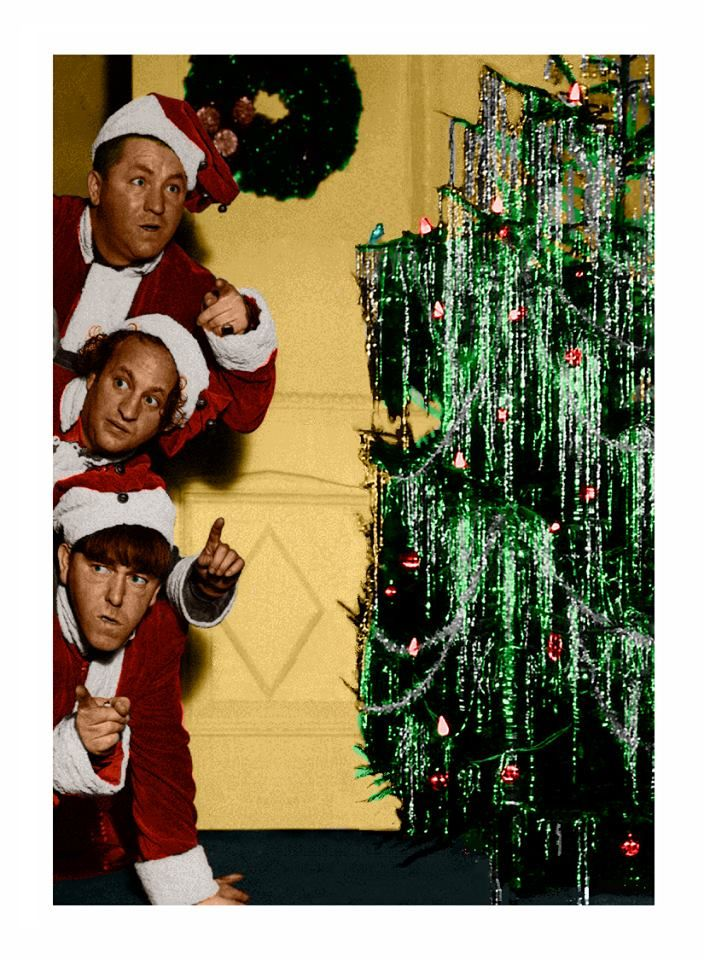
\includegraphics[max width=.95\textwidth,
            max height=0.55\textheight]{Images/stoogesxmas.jpg}
    \end{center}
    \pause
    It turns out that they do.
\end{frame}

\begin{frame}
    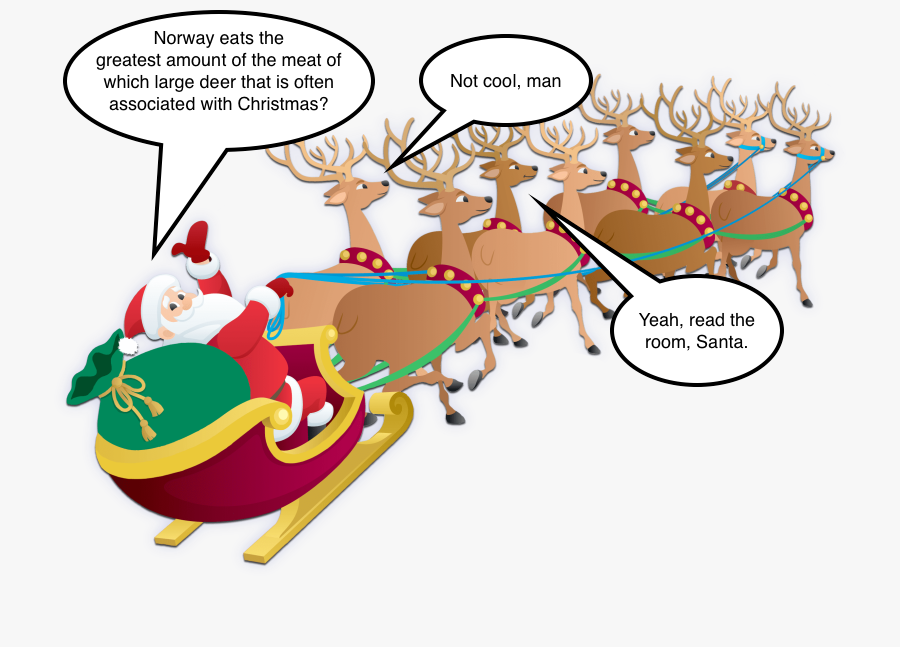
\includegraphics[max width=.95\textwidth,
        max height=.95\textheight]{Images/santasleigh.png}
\end{frame}

\begingroup{}
\begingroup{}
\begin{frame}[t]{Categories}
    This week, you'll be answering questions in the following categories:
    \begin{enumerate}
        \item Board Games
        \item Companies That Are No More
        \item Famous Foreign-Language Literary Works
        \item Newspapers and Magazines
        \item One of the things this city is famous for is\ldots
        \item Winter Sports
        \item Cartoons and the Funny Pages
        \item Specialized Words II
        \item Other Things that Happened in 2020
        \item Movies From Their Stills
        \item Bonus Round
    \end{enumerate}
\end{frame}
\endgroup{}

\begingroup{}
\begin{frame}
    \vfill{}
    \begin{beamercolorbox}[sep=8pt,center,shadow=true,rounded=true]{title}
        \usebeamerfont{title}Good luck everyone! And have fun!
    \end{beamercolorbox}
    \vfill{}
\end{frame}
\endgroup{}
\def\thisSectionName{Board Games}
\section{Round 1}
\subsection*{Q1}
\begin{frame}[t]{Round 1 --- Board Games --- \mbox{Question 1}}
    \vspace{-0.5em}
    \begin{block}{Question}
        In \emph{Monopoly}, what is the other half of the property group that contains Park Place?
    \end{block}
\end{frame}
\subsection*{Q2}
\begin{frame}[t]{Round 1 --- Board Games --- \mbox{Question 2}}
    \vspace{-0.5em}
    \begin{block}{Question}
        In which board game is the winner the first player to \emph{bear off}\,?
    \end{block}
\end{frame}
\subsection*{Q3}
\begin{frame}[t]{Round 1 --- Board Games --- \mbox{Question 3}}
    \vspace{-0.5em}
    \begin{block}{Question}
        How many rooms are there in the game \emph{Clue}? (Don't count the hallways or the staircase.)
    \end{block}
\end{frame}
\subsection*{Q4}
\begin{frame}[t]{Round 1 --- Board Games --- \mbox{Question 4}}
    \vspace{-0.5em}
    \begin{block}{Question}
        Which board game's tagline is ``Trade, build, settle''?
    \end{block}
\end{frame}
\subsection*{Q5}
\begin{frame}[t]{Round 1 --- Board Games --- \mbox{Question 5}}
    \vspace{-0.5em}
    \begin{block}{Question}
        What was the name of the first artificial intelligence to defeat a professional Go player without a handicap?
    \end{block}
\end{frame}
\subsection*{Q6}
\begin{frame}[t]{Round 1 --- Board Games --- \mbox{Question 6}}
    \vspace{-0.5em}
    \begin{block}{Question}
        On \emph{Seinfeld}, what board game were Kramer and Newman playing on the subway when Kramer said, ``The Ukraine is weak''?
    \end{block}
\end{frame}
\subsection*{Q7}
\begin{frame}[t]{Round 1 --- Board Games --- \mbox{Question 7}}
    \vspace{-0.5em}
    \begin{columns}[T,totalwidth=\linewidth]
        \begin{column}{0.32\linewidth}
            \begin{block}{Question}
                Which board game is pictured here?
            \end{block}
        \end{column}
        \begin{column}{0.65\linewidth}
            \begin{center}
                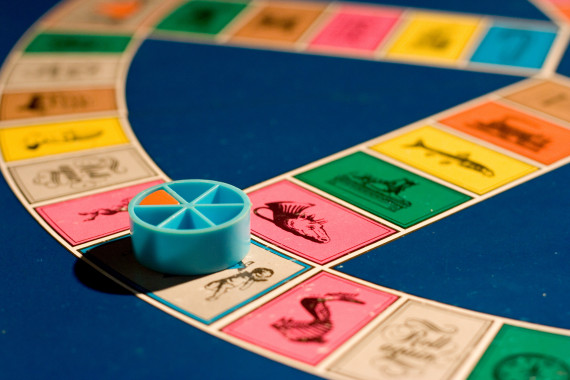
\includegraphics[max width=0.95\textwidth,max height=0.7\textheight]{{Images/trivialpursuit}.jpg}
            \end{center}
        \end{column}
    \end{columns}
\end{frame}
\subsection*{Q8}
\begin{frame}[t]{Round 1 --- Board Games --- \mbox{Question 8}}
    \vspace{-0.5em}
    \begin{block}{Question}
        In standard chess notation, what does O--O--O denote?
    \end{block}
\end{frame}
\subsection*{Q9}
\begin{frame}[t]{Round 1 --- Board Games --- \mbox{Question 9}}
    \vspace{-0.5em}
    \begin{block}{Question}
        Which children's board game was invented in 1948 by a polio patient and was first played by other patients in the polio ward, who suggested that the inventor submit the game to the Milton Bradley Company?
    \end{block}
\end{frame}
\subsection*{Q10}
\begin{frame}[t]{Round 1 --- Board Games --- \mbox{Question 10}}
    \vspace{-0.5em}
    \begin{block}{Question}
        To within five years, in what year was the Milton Bradley Company founded?
    \end{block}
\end{frame}
\subsection{Answers}
\begin{frame}[t]{Round 1 --- Board Games --- \mbox{Answer 1}}
    \vspace{-0.5em}
    \begin{block}{Question}
        In \emph{Monopoly}, what is the other half of the property group that contains Park Place?
    \end{block}

    \visible<2->{
        \begin{columns}[T,totalwidth=\linewidth]
            \begin{column}{0.32\linewidth}
                \begin{block}{Answer}
                    Boardwalk
                \end{block}
            \end{column}
            \begin{column}{0.65\linewidth}
                \begin{center}
                    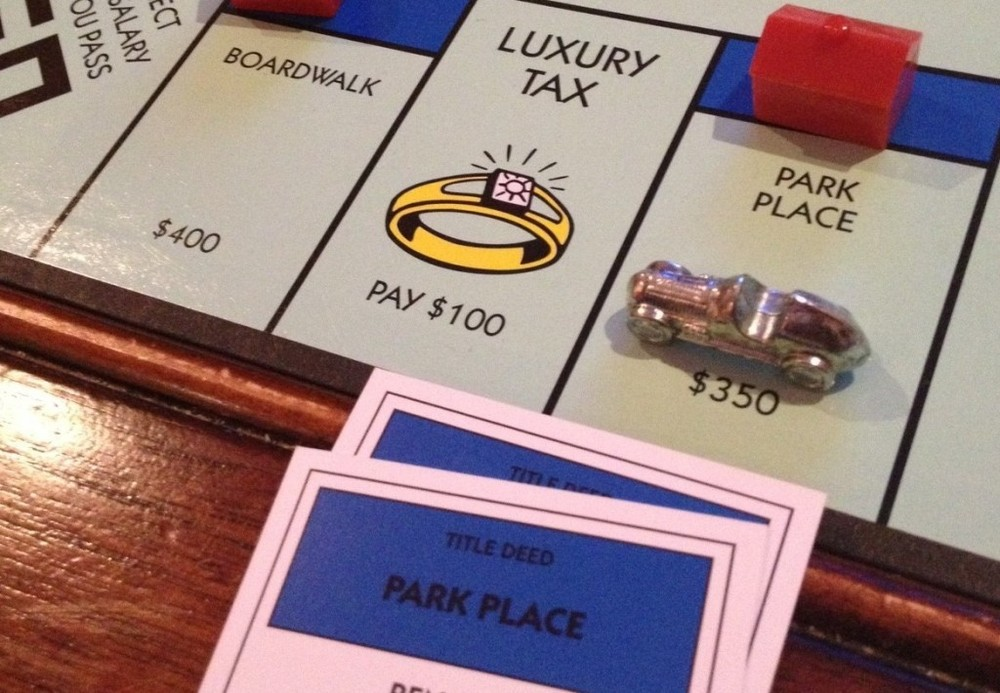
\includegraphics[max width=0.95\textwidth,
                        max height=0.53000\textheight]{{Images/boardwalk}.jpg}
                \end{center}
            \end{column}
        \end{columns}
    }
\end{frame}
\begin{frame}[t]{Round 1 --- Board Games --- \mbox{Answer 2}}
    \vspace{-0.5em}
    \begin{block}{Question}
        In which board game is the winner the first player to \emph{bear off}\,?
    \end{block}

    \visible<2->{
        \begin{columns}[T,totalwidth=\linewidth]
            \begin{column}{0.32\linewidth}
                \begin{block}{Answer}
                    Backgammon
                \end{block}
            \end{column}
            \begin{column}{0.65\linewidth}
                \begin{center}
                    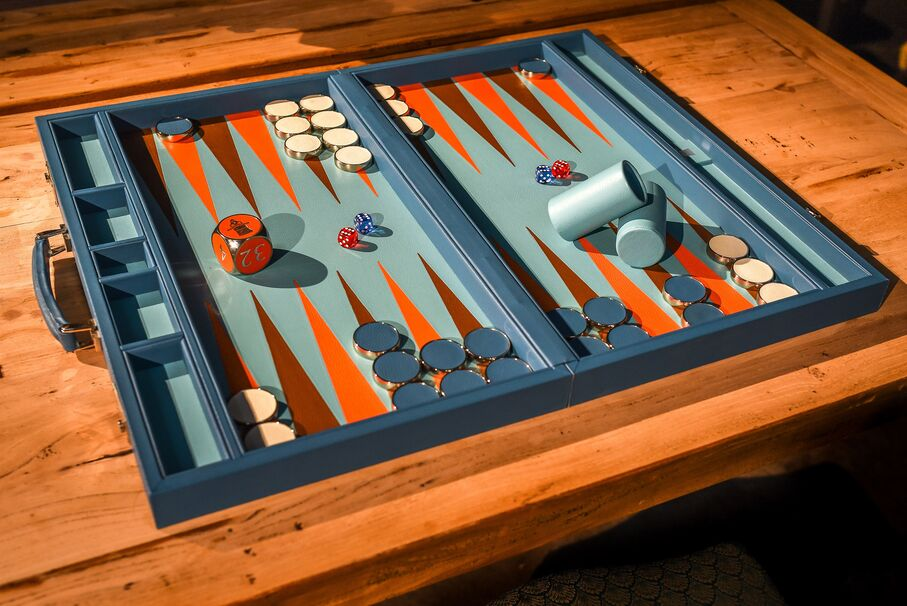
\includegraphics[max width=0.95\textwidth,
                        max height=0.53000\textheight]{{Images/backgammon}.jpg}
                \end{center}
            \end{column}
        \end{columns}
    }
\end{frame}
\begin{frame}[t]{Round 1 --- Board Games --- \mbox{Answer 3}}
    \vspace{-0.5em}
    \begin{block}{Question}
        How many rooms are there in the game \emph{Clue}? (Don't count the hallways or the staircase.)
    \end{block}

    \visible<2->{
        \begin{columns}[T,totalwidth=\linewidth]
            \begin{column}{0.32\linewidth}
                \begin{block}{Answer}
                    Nine
                \end{block}
            \end{column}
            \begin{column}{0.65\linewidth}
                \begin{center}
                    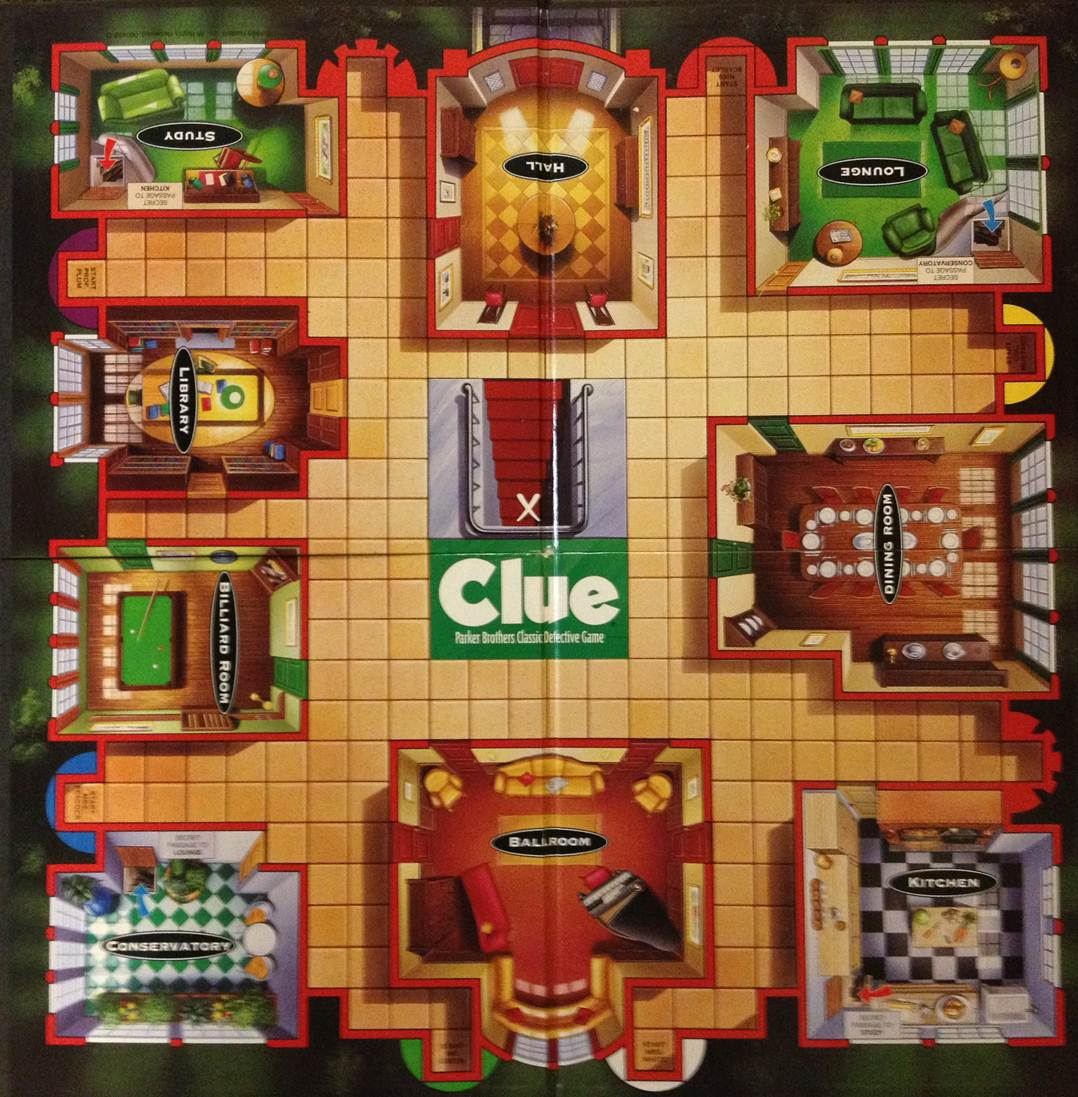
\includegraphics[max width=0.95\textwidth,
                        max height=0.53000\textheight]{{Images/clueboard}.jpg}
                \end{center}
            \end{column}
        \end{columns}
    }
\end{frame}
\begin{frame}[t]{Round 1 --- Board Games --- \mbox{Answer 4}}
    \vspace{-0.5em}
    \begin{block}{Question}
        Which board game's tagline is ``Trade, build, settle''?
    \end{block}

    \visible<2->{
        \begin{columns}[T,totalwidth=\linewidth]
            \begin{column}{0.32\linewidth}
                \begin{block}{Answer}
                    \emph{Settlers of Catan} / \emph{Settlers} / \emph{Catan}
                \end{block}
            \end{column}
            \begin{column}{0.65\linewidth}
                \begin{center}
                    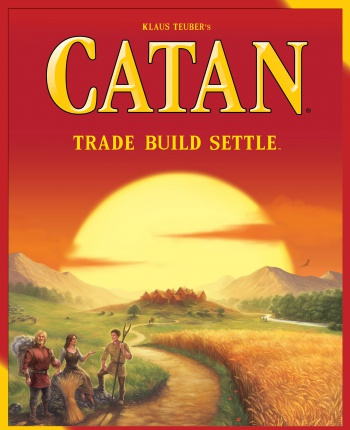
\includegraphics[max width=0.95\textwidth,
                        max height=0.53000\textheight]{{Images/catan}.jpg}
                \end{center}
            \end{column}
        \end{columns}
    }
\end{frame}
\begin{frame}[t]{Round 1 --- Board Games --- \mbox{Answer 5}}
    \vspace{-0.5em}
    \begin{block}{Question}
        What was the name of the first artificial intelligence to defeat a professional Go player without a handicap?
    \end{block}

    \visible<2->{
        \begin{columns}[T,totalwidth=\linewidth]
            \begin{column}{0.32\linewidth}
                \begin{block}{Answer}
                    AlphaGo
                \end{block}
            \end{column}
            \begin{column}{0.65\linewidth}
                \begin{center}
                    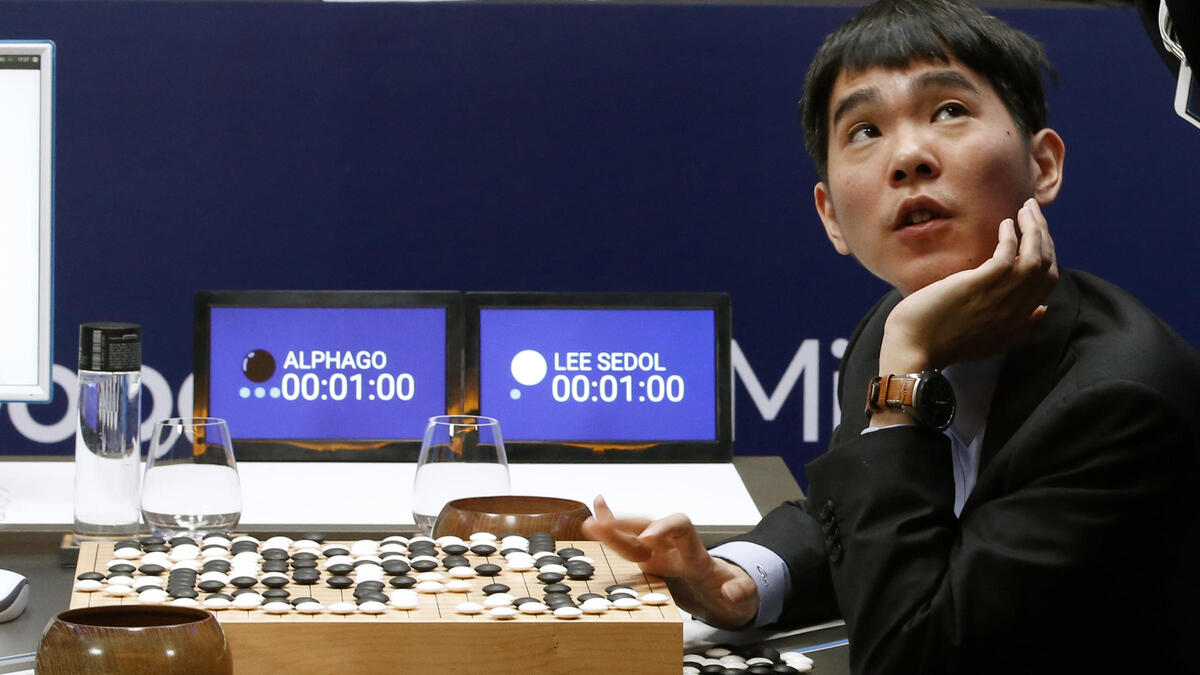
\includegraphics[max width=0.95\textwidth,
                        max height=0.48000\textheight]{{Images/alphago}.jpg}
                \end{center}
            \end{column}
        \end{columns}
    }
\end{frame}
\begin{frame}[t]{Round 1 --- Board Games --- \mbox{Answer 6}}
    \vspace{-0.5em}
    \begin{block}{Question}
        On \emph{Seinfeld}, what board game were Kramer and Newman playing on the subway when Kramer said, ``The Ukraine is weak''?
    \end{block}

    \visible<2->{
        \begin{columns}[T,totalwidth=\linewidth]
            \begin{column}{0.32\linewidth}
                \begin{block}{Answer}
                    \emph{Risk}
                \end{block}
            \end{column}
            \begin{column}{0.65\linewidth}
                \begin{center}
                    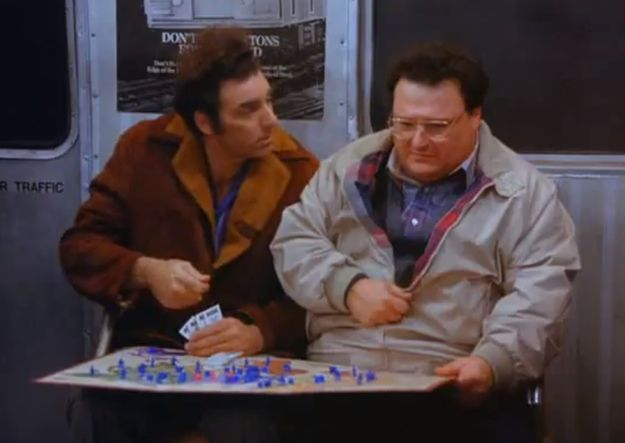
\includegraphics[max width=0.95\textwidth,
                        max height=0.48000\textheight]{{Images/ukraine}.jpg}
                \end{center}
            \end{column}
        \end{columns}
    }
\end{frame}
\begin{frame}[t]{Round 1 --- Board Games --- \mbox{Answer 7}}
    \vspace{-0.5em}
    \begin{columns}[T,totalwidth=\linewidth]
        \begin{column}{0.32\linewidth}
            \begin{block}{Question}
                Which board game is pictured here?
            \end{block}
            \visible<2->{
                \begin{block}{Answer}
                    \emph{Trivial Pursuit}
                \end{block}
            }
        \end{column}
        \begin{column}{0.65\linewidth}
            \begin{center}
                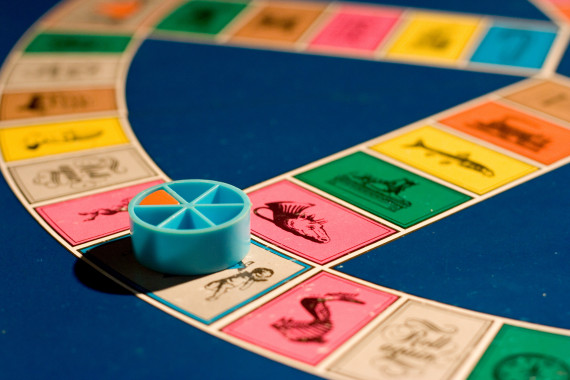
\includegraphics[max width=0.95\textwidth,max height=0.7\textheight]{{Images/trivialpursuit}.jpg}
            \end{center}
        \end{column}
    \end{columns}
\end{frame}
\begin{frame}[t]{Round 1 --- Board Games --- \mbox{Answer 8}}
    \vspace{-0.5em}
    \begin{block}{Question}
        In standard chess notation, what does O--O--O denote?
    \end{block}

    \visible<2->{
        \begin{columns}[T,totalwidth=\linewidth]
            \begin{column}{0.32\linewidth}
                \begin{block}{Answer}
                    A queenside castle
                \end{block}
            \end{column}
            \begin{column}{0.65\linewidth}
                \begin{center}
                    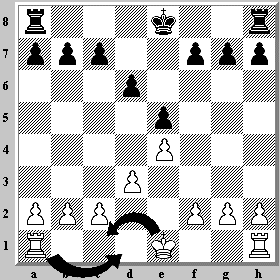
\includegraphics[max width=0.95\textwidth,
                        max height=0.53000\textheight]{{Images/queenside}.png}
                \end{center}
            \end{column}
        \end{columns}
    }
\end{frame}
\begin{frame}[t]{Round 1 --- Board Games --- \mbox{Answer 9}}
    \vspace{-0.5em}
    \begin{block}{Question}
        Which children's board game was invented in 1948 by a polio patient and was first played by other patients in the polio ward, who suggested that the inventor submit the game to the Milton Bradley Company?
    \end{block}

    \visible<2->{
        \begin{columns}[T,totalwidth=\linewidth]
            \begin{column}{0.32\linewidth}
                \begin{block}{Answer}
                    \emph{Candy Land}
                \end{block}
            \end{column}
            \begin{column}{0.65\linewidth}
                \begin{center}
                    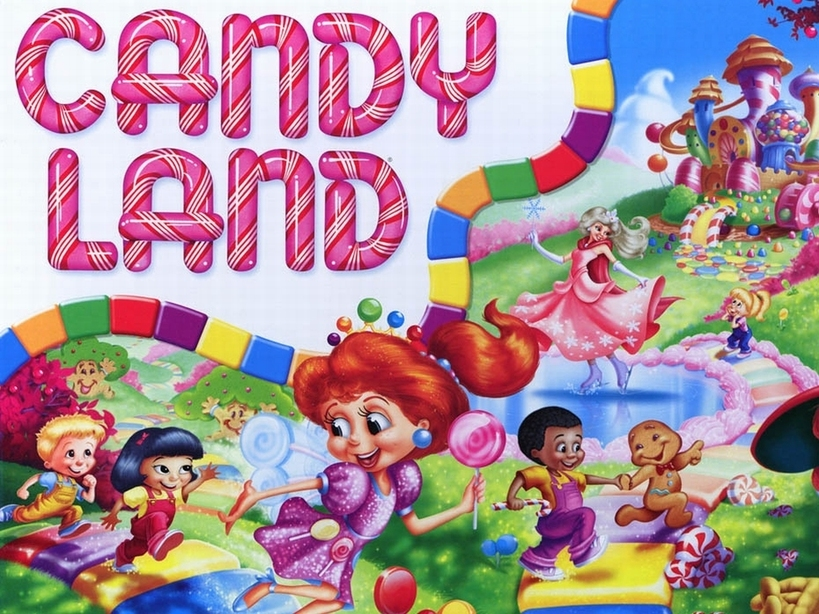
\includegraphics[max width=0.95\textwidth,
                        max height=0.38000\textheight]{{Images/candyland}.jpg}
                \end{center}
            \end{column}
        \end{columns}
    }
\end{frame}
\begin{frame}[t]{Round 1 --- Board Games --- \mbox{Answer 10}}
    \vspace{-0.5em}
    \begin{block}{Question}
        To within five years, in what year was the Milton Bradley Company founded?
    \end{block}

    \visible<2->{
        \begin{columns}[T,totalwidth=\linewidth]
            \begin{column}{0.32\linewidth}
                \begin{block}{Answer}
                    1860 (1855-1865 will be accepted)
                \end{block}
            \end{column}
            \begin{column}{0.65\linewidth}
                \begin{center}
                    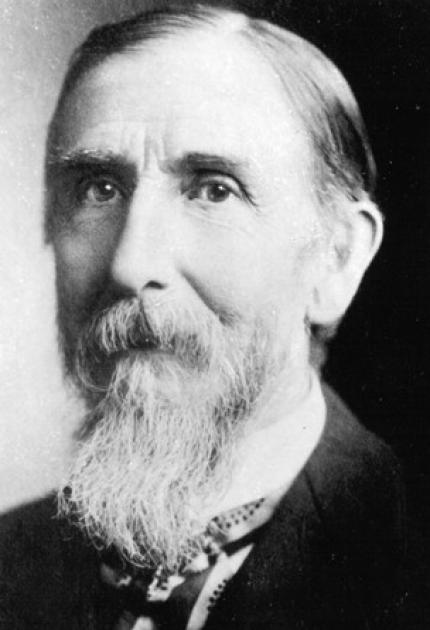
\includegraphics[max width=0.95\textwidth,
                        max height=0.53000\textheight]{{Images/bradley}.jpg}
                \end{center}
            \end{column}
        \end{columns}
    }
\end{frame}
\def\thisSectionName{Companies That Are No More}
\section{Round 2}
\subsection*{Q1}
\begin{frame}[t]{Round 2 --- Companies That Are No More --- \mbox{Question 1}}
    \vspace{-0.5em}
    \begin{block}{Question}
        Which sporting goods store, founded in New York City in 1889, can you no longer go to because they declared bankruptcy in March of this year?
    \end{block}
\end{frame}
\subsection*{Q2}
\begin{frame}[t]{Round 2 --- Companies That Are No More --- \mbox{Question 2}}
    \vspace{-0.5em}
    \begin{block}{Question}
        When Steve Jobs was booted from Apple, he founded his own computer and software company, which was later acquired by Apple. What was the name of this company?
    \end{block}
\end{frame}
\subsection*{Q3}
\begin{frame}[t]{Round 2 --- Companies That Are No More --- \mbox{Question 3}}
    \vspace{-0.5em}
    \begin{block}{Question}
        What was the name of the ``Big Five'' accounting firm that helped cover up the financial issues plaguing the Enron Corporation and was subsequently dissolved?
    \end{block}
\end{frame}
\subsection*{Q4}
\begin{frame}[t]{Round 2 --- Companies That Are No More --- \mbox{Question 4}}
    \vspace{-0.5em}
    \begin{block}{Question}
        Which large US airline that folded in 1991 was known for their ``Clipper'' flights, one of which was the first trans-Atlantic passenger flight?
    \end{block}
\end{frame}
\subsection*{Q5}
\begin{frame}[t]{Round 2 --- Companies That Are No More --- \mbox{Question 5}}
    \vspace{-0.5em}
    \begin{block}{Question}
        On September 15, 2008, which investment bank filed for bankruptcy in what is still the largest Chapter 11 filing in history?
    \end{block}
\end{frame}
\subsection*{Q6}
\begin{frame}[t]{Round 2 --- Companies That Are No More --- \mbox{Question 6}}
    \vspace{-0.5em}
    \begin{block}{Question}
        Which defunct grocery store chain provided the lead singer of The Waitresses with the world's smallest turkey in the song \emph{Christmas Wrapping}?
    \end{block}
\end{frame}
\subsection*{Q7}
\begin{frame}[t]{Round 2 --- Companies That Are No More --- \mbox{Question 7}}
    \vspace{-0.5em}
    \begin{block}{Question}
        ``G'', it's too bad ``U'' won't ``C'' any locations of which former chain of toy stores that filed for Chapter 11 in 2017?
    \end{block}
\end{frame}
\subsection*{Q8}
\begin{frame}[t]{Round 2 --- Companies That Are No More --- \mbox{Question 8}}
    \vspace{-0.5em}
    \begin{block}{Question}
        ``Where the Streets are Paved with Bargains'' was the slogan of which chain of electronics stores that went out of business in 2008?
    \end{block}
\end{frame}
\subsection*{Q9}
\begin{frame}[t]{Round 2 --- Companies That Are No More --- \mbox{Question 9}}
    \vspace{-0.5em}
    \begin{block}{Question}
        Which former restaurant chain --- one of the first nationwide restaurant chains in the US --- pivoted into the hotel/motel business, and now no longer operates any restaurants? (Their hotels and motels are doing fine; it's the restaurants that are no more.)
    \end{block}
\end{frame}
\subsection*{Q10}
\begin{frame}[t]{Round 2 --- Companies That Are No More --- \mbox{Question 10}}
    \vspace{-0.5em}
    \begin{block}{Question}
        Which software company created the most popular web browsers of the `90s, but ultimately went out of business because it could not compete with Microsoft's free Internet Explorer? (Its browser's code lives in on Mozilla's Firefox browser.)
    \end{block}
\end{frame}
\subsection{Answers}
\begin{frame}[t]{Round 2 --- Companies That Are No More --- \mbox{Answer 1}}
    \vspace{-0.5em}
    \begin{block}{Question}
        Which sporting goods store, founded in New York City in 1889, can you no longer go to because they declared bankruptcy in March of this year?
    \end{block}

    \visible<2->{
        \begin{columns}[T,totalwidth=\linewidth]
            \begin{column}{0.32\linewidth}
                \begin{block}{Answer}
                    Modell's
                \end{block}
            \end{column}
            \begin{column}{0.65\linewidth}
                \begin{center}
                    
\includegraphics[max width=0.95\textwidth,
                        max height=0.48000\textheight]{{Images/modells}.png}
                \end{center}
            \end{column}
        \end{columns}
    }
\end{frame}
\begin{frame}[t]{Round 2 --- Companies That Are No More --- \mbox{Answer 2}}
    \vspace{-0.5em}
    \begin{block}{Question}
        When Steve Jobs was booted from Apple, he founded his own computer and software company, which was later acquired by Apple. What was the name of this company?
    \end{block}

    \visible<2->{
        \begin{columns}[T,totalwidth=\linewidth]
            \begin{column}{0.32\linewidth}
                \begin{block}{Answer}
                    NeXT
                \end{block}
            \end{column}
            \begin{column}{0.65\linewidth}
                \begin{center}
                    
\includegraphics[max width=0.95\textwidth,
                        max height=0.43000\textheight]{{Images/next}.png}
                \end{center}
            \end{column}
        \end{columns}
    }
\end{frame}
\begin{frame}[t]{Round 2 --- Companies That Are No More --- \mbox{Answer 3}}
    \vspace{-0.5em}
    \begin{block}{Question}
        What was the name of the ``Big Five'' accounting firm that helped cover up the financial issues plaguing the Enron Corporation and was subsequently dissolved?
    \end{block}

    \visible<2->{
        \begin{columns}[T,totalwidth=\linewidth]
            \begin{column}{0.32\linewidth}
                \begin{block}{Answer}
                    Arthur Andersen
                \end{block}
            \end{column}
            \begin{column}{0.65\linewidth}
                \begin{center}
                    
\includegraphics[max width=0.95\textwidth,
                        max height=0.43000\textheight]{{Images/arthuranderson}.png}
                \end{center}
            \end{column}
        \end{columns}
    }
\end{frame}
\begin{frame}[t]{Round 2 --- Companies That Are No More --- \mbox{Answer 4}}
    \vspace{-0.5em}
    \begin{block}{Question}
        Which large US airline that folded in 1991 was known for their ``Clipper'' flights, one of which was the first trans-Atlantic passenger flight?
    \end{block}

    \visible<2->{
        \begin{columns}[T,totalwidth=\linewidth]
            \begin{column}{0.32\linewidth}
                \begin{block}{Answer}
                    Pan Am / Pan American Airlines
                \end{block}
            \end{column}
            \begin{column}{0.65\linewidth}
                \begin{center}
                    
\includegraphics[max width=0.95\textwidth,
                        max height=0.48000\textheight]{{Images/panam}.png}
                \end{center}
            \end{column}
        \end{columns}
    }
\end{frame}
\begin{frame}[t]{Round 2 --- Companies That Are No More --- \mbox{Answer 5}}
    \vspace{-0.5em}
    \begin{block}{Question}
        On September 15, 2008, which investment bank filed for bankruptcy in what is still the largest Chapter 11 filing in history?
    \end{block}
    \visible<2->{
        \begin{block}{Answer}
            Lehman Brothers
        \end{block}
    }
\end{frame}
\begin{frame}[t]{Round 2 --- Companies That Are No More --- \mbox{Answer 6}}
    \vspace{-0.5em}
    \begin{block}{Question}
        Which defunct grocery store chain provided the lead singer of The Waitresses with the world's smallest turkey in the song \emph{Christmas Wrapping}?
    \end{block}

    \visible<2->{
        \begin{columns}[T,totalwidth=\linewidth]
            \begin{column}{0.32\linewidth}
                \begin{block}{Answer}
                    A\&P
                \end{block}
            \end{column}
            \begin{column}{0.65\linewidth}
                \begin{center}
                    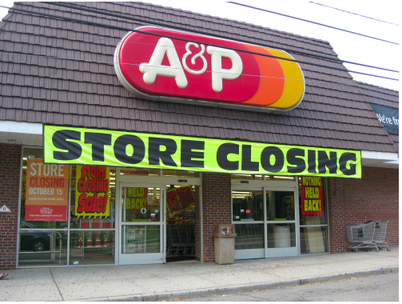
\includegraphics[max width=0.95\textwidth,
                        max height=0.48000\textheight]{{Images/ap}.jpg}
                \end{center}
            \end{column}
        \end{columns}
    }
\end{frame}
\begin{frame}[t]{Round 2 --- Companies That Are No More --- \mbox{Answer 7}}
    \vspace{-0.5em}
    \begin{block}{Question}
        ``G'', it's too bad ``U'' won't ``C'' any locations of which former chain of toy stores that filed for Chapter 11 in 2017?
    \end{block}

    \visible<2->{
        \begin{columns}[T,totalwidth=\linewidth]
            \begin{column}{0.32\linewidth}
                \begin{block}{Answer}
                    Toys ``R'' Us
                \end{block}
            \end{column}
            \begin{column}{0.65\linewidth}
                \begin{center}
                    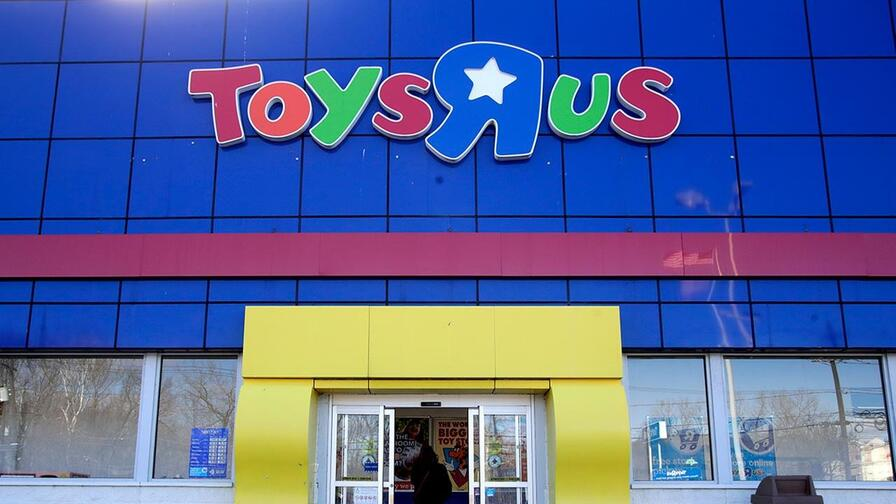
\includegraphics[max width=0.95\textwidth,
                        max height=0.48000\textheight]{{Images/toysrus}.jpg}
                \end{center}
            \end{column}
        \end{columns}
    }
\end{frame}
\begin{frame}[t]{Round 2 --- Companies That Are No More --- \mbox{Answer 8}}
    \vspace{-0.5em}
    \begin{block}{Question}
        ``Where the Streets are Paved with Bargains'' was the slogan of which chain of electronics stores that went out of business in 2008?
    \end{block}

    \visible<2->{
        \begin{columns}[T,totalwidth=\linewidth]
            \begin{column}{0.32\linewidth}
                \begin{block}{Answer}
                    Circuit City
                \end{block}
            \end{column}
            \begin{column}{0.65\linewidth}
                \begin{center}
                    
\includegraphics[max width=0.95\textwidth,
                        max height=0.48000\textheight]{{Images/circuitcity}.jpg}
                \end{center}
            \end{column}
        \end{columns}
    }
\end{frame}
\begin{frame}[t]{Round 2 --- Companies That Are No More --- \mbox{Answer 9}}
    \vspace{-0.5em}
    \begin{block}{Question}
        Which former restaurant chain --- one of the first nationwide restaurant chains in the US --- pivoted into the hotel/motel business, and now no longer operates any restaurants? (Their hotels and motels are doing fine; it's the restaurants that are no more.)
    \end{block}

    \visible<2->{
        \begin{columns}[T,totalwidth=\linewidth]
            \begin{column}{0.32\linewidth}
                \begin{block}{Answer}
                    Howard Johnson / HoJo
                \end{block}
            \end{column}
            \begin{column}{0.65\linewidth}
                \begin{center}
                    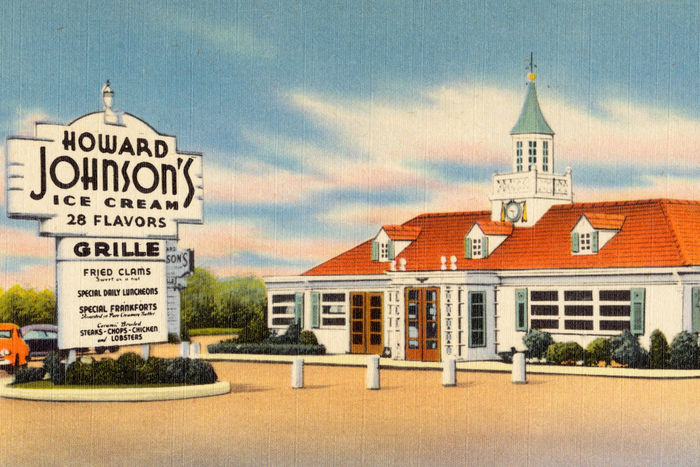
\includegraphics[max width=0.95\textwidth,
                        max height=0.33000\textheight]{{Images/hojos}.jpg}
                \end{center}
            \end{column}
        \end{columns}
    }
\end{frame}
\begin{frame}[t]{Round 2 --- Companies That Are No More --- \mbox{Answer 10}}
    \vspace{-0.5em}
    \begin{block}{Question}
        Which software company created the most popular web browsers of the `90s, but ultimately went out of business because it could not compete with Microsoft's free Internet Explorer? (Its browser's code lives in on Mozilla's Firefox browser.)
    \end{block}

    \visible<2->{
        \begin{columns}[T,totalwidth=\linewidth]
            \begin{column}{0.32\linewidth}
                \begin{block}{Answer}
                    Netscape
                \end{block}
            \end{column}
            \begin{column}{0.65\linewidth}
                \begin{center}
                    
\includegraphics[max width=0.95\textwidth,
                        max height=0.38000\textheight]{{Images/netscape}.png}
                \end{center}
            \end{column}
        \end{columns}
    }
\end{frame}
\def\thisSectionName{Famous Foreign-Language Literary Works}
\section{Round 3}
\subsection*{Q1}
\begin{frame}[t]{Round 3 --- Famous Foreign-Language Literary Works --- \mbox{Question 1}}
    \vspace{-0.5em}
    \begin{block}{Question}
        \emph{L'Étranger}
    \end{block}
\end{frame}
\subsection*{Q2}
\begin{frame}[t]{Round 3 --- Famous Foreign-Language Literary Works --- \mbox{Question 2}}
    \vspace{-0.5em}
    \begin{block}{Question}
        \emph{Im Westen nichts Neues}
    \end{block}
\end{frame}
\subsection*{Q3}
\begin{frame}[t]{Round 3 --- Famous Foreign-Language Literary Works --- \mbox{Question 3}}
    \vspace{-0.5em}
    \begin{block}{Question}
        \emph{孙子兵法} (S\=unzi b\={\i}ngf\v a)
    \end{block}
\end{frame}
\subsection*{Q4}
\begin{frame}[t]{Round 3 --- Famous Foreign-Language Literary Works --- \mbox{Question 4}}
    \vspace{-0.5em}
    \begin{block}{Question}
        \emph{`\textIota\textlambda\textiota\textalpha\textvarsigma{}}
    \end{block}
\end{frame}
\subsection*{Q5}
\begin{frame}[t]{Round 3 --- Famous Foreign-Language Literary Works --- \mbox{Question 5}}
    \vspace{-0.5em}
    \begin{block}{Question}
        \emph{Nesnesitelná lehkost bytí} (Czech)
    \end{block}
\end{frame}
\subsection*{Q6}
\begin{frame}[t]{Round 3 --- Famous Foreign-Language Literary Works --- \mbox{Question 6}}
    \vspace{-0.5em}
    \begin{block}{Question}
        \emph{À la recherche du temps perdu}
    \end{block}
\end{frame}
\subsection*{Q7}
\begin{frame}[t]{Round 3 --- Famous Foreign-Language Literary Works --- \mbox{Question 7}}
    \vspace{-0.5em}
    \begin{block}{Question}
        \emph{Les Faux-monnayeurs}
    \end{block}
\end{frame}
\subsection*{Q8}
\begin{frame}[t]{Round 3 --- Famous Foreign-Language Literary Works --- \mbox{Question 8}}
    \vspace{-0.5em}
    \begin{block}{Question}
        \emph{Der Proce{\ss}}
    \end{block}
\end{frame}
\subsection*{Q9}
\begin{frame}[t]{Round 3 --- Famous Foreign-Language Literary Works --- \mbox{Question 9}}
    \vspace{-0.5em}
    \begin{block}{Question}
        \emph{La condition humaine}
    \end{block}
\end{frame}
\subsection*{Q10}
\begin{frame}[t]{Round 3 --- Famous Foreign-Language Literary Works --- \mbox{Question 10}}
    \vspace{-0.5em}
    \begin{block}{Question}
        \emph{Sei personaggi in cerca d'autore}
    \end{block}
\end{frame}
\subsection{Answers}
\begin{frame}[t]{Round 3 --- Famous Foreign-Language Literary Works --- \mbox{Answer 1}}
    \vspace{-0.5em}
    \begin{block}{Question}
        \emph{L'Étranger}
    \end{block}

    \visible<2->{
        \begin{columns}[T,totalwidth=\linewidth]
            \begin{column}{0.32\linewidth}
                \begin{block}{Answer}
                    \emph{The Stranger} (Camus)
                \end{block}
            \end{column}
            \begin{column}{0.65\linewidth}
                \begin{center}
                    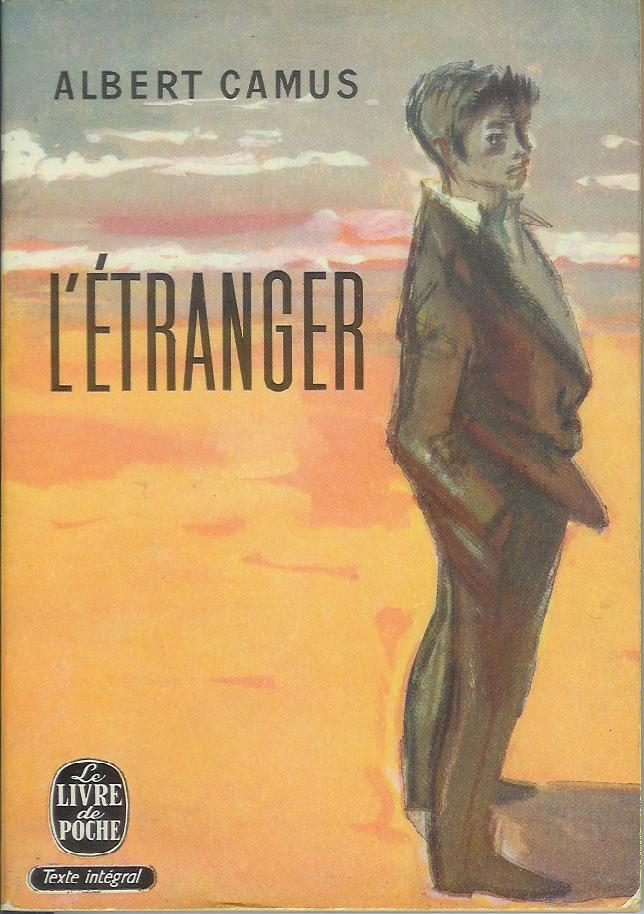
\includegraphics[max width=0.95\textwidth,
                        max height=0.58000\textheight]{{Images/letranger}.jpg}
                \end{center}
            \end{column}
        \end{columns}
    }
\end{frame}
\begin{frame}[t]{Round 3 --- Famous Foreign-Language Literary Works --- \mbox{Answer 2}}
    \vspace{-0.5em}
    \begin{block}{Question}
        \emph{Im Westen nichts Neues}
    \end{block}

    \visible<2->{
        \begin{columns}[T,totalwidth=\linewidth]
            \begin{column}{0.32\linewidth}
                \begin{block}{Answer}
                    \emph{All Quiet on the Western Front} (Remarque)
                \end{block}
            \end{column}
            \begin{column}{0.65\linewidth}
                \begin{center}
                    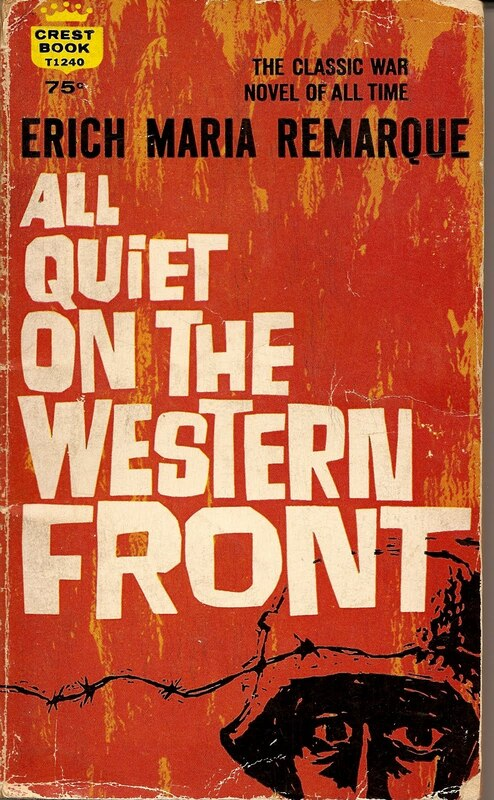
\includegraphics[max width=0.95\textwidth,
                        max height=0.58000\textheight]{{Images/allquiet}.jpg}
                \end{center}
            \end{column}
        \end{columns}
    }
\end{frame}
\begin{frame}[t]{Round 3 --- Famous Foreign-Language Literary Works --- \mbox{Answer 3}}
    \vspace{-0.5em}
    \begin{block}{Question}
        \emph{孙子兵法} (S\=unzi b\={\i}ngf\v a)
    \end{block}

    \visible<2->{
        \begin{columns}[T,totalwidth=\linewidth]
            \begin{column}{0.32\linewidth}
                \begin{block}{Answer}
                    \emph{The Art of War} (by Sun Tzu)
                \end{block}
            \end{column}
            \begin{column}{0.65\linewidth}
                \begin{center}
                    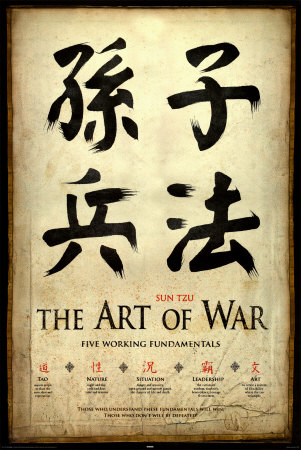
\includegraphics[max width=0.95\textwidth,
                        max height=0.58000\textheight]{{Images/artofwar}.jpg}
                \end{center}
            \end{column}
        \end{columns}
    }
\end{frame}
\begin{frame}[t]{Round 3 --- Famous Foreign-Language Literary Works --- \mbox{Answer 4}}
    \vspace{-0.5em}
    \begin{block}{Question}
        \emph{`\textIota\textlambda\textiota\textalpha\textvarsigma{}}
    \end{block}

    \visible<2->{
        \begin{columns}[T,totalwidth=\linewidth]
            \begin{column}{0.32\linewidth}
                \begin{block}{Answer}
                    \emph{The Iliad} (Homer (maybe))
                \end{block}
            \end{column}
            \begin{column}{0.65\linewidth}
                \begin{center}
                    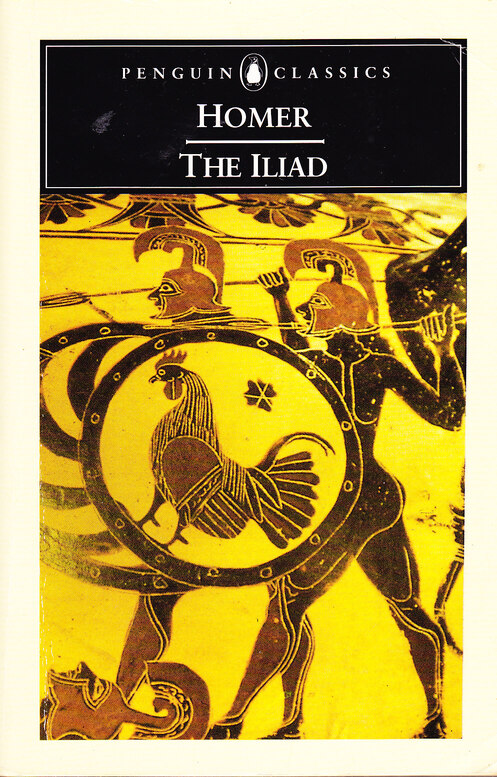
\includegraphics[max width=0.95\textwidth,
                        max height=0.53000\textheight]{{Images/iliad}.jpg}
                \end{center}
            \end{column}
        \end{columns}
    }
\end{frame}
\begin{frame}[t]{Round 3 --- Famous Foreign-Language Literary Works --- \mbox{Answer 5}}
    \vspace{-0.5em}
    \begin{block}{Question}
        \emph{Nesnesitelná lehkost bytí} (Czech)
    \end{block}

    \visible<2->{
        \begin{columns}[T,totalwidth=\linewidth]
            \begin{column}{0.32\linewidth}
                \begin{block}{Answer}
                    \emph{The Unbearable Lightness of Being} (Kundera)
                \end{block}
            \end{column}
            \begin{column}{0.65\linewidth}
                \begin{center}
                    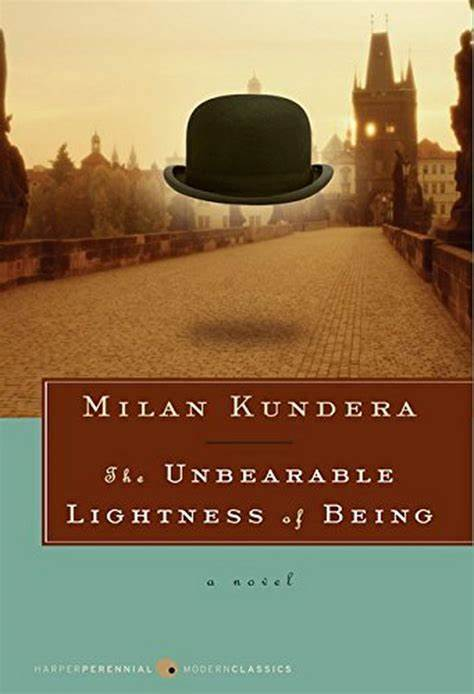
\includegraphics[max width=0.95\textwidth,
                        max height=0.58000\textheight]{{Images/lightness}.jpeg}
                \end{center}
            \end{column}
        \end{columns}
    }
\end{frame}
\begin{frame}[t]{Round 3 --- Famous Foreign-Language Literary Works --- \mbox{Answer 6}}
    \vspace{-0.5em}
    \begin{block}{Question}
        \emph{À la recherche du temps perdu}
    \end{block}

    \visible<2->{
        \begin{columns}[T,totalwidth=\linewidth]
            \begin{column}{0.32\linewidth}
                \begin{block}{Answer}
                    \emph{In Search of Lost Time} / \emph{Remembrance of Things Past} (Proust)
                \end{block}
            \end{column}
            \begin{column}{0.65\linewidth}
                \begin{center}
                    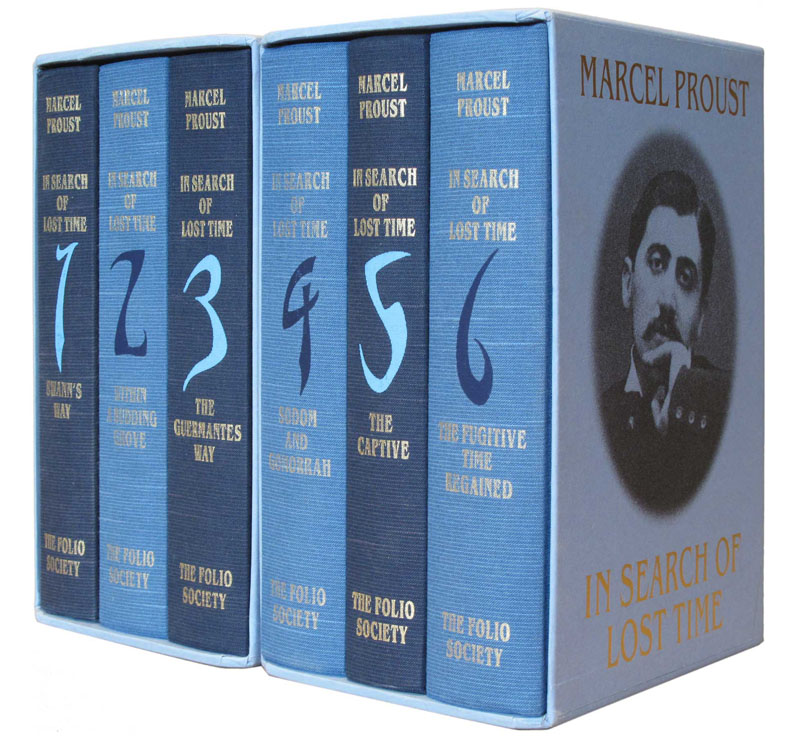
\includegraphics[max width=0.95\textwidth,
                        max height=0.58000\textheight]{{Images/searchoflosttime}.jpg}
                \end{center}
            \end{column}
        \end{columns}
    }
\end{frame}
\begin{frame}[t]{Round 3 --- Famous Foreign-Language Literary Works --- \mbox{Answer 7}}
    \vspace{-0.5em}
    \begin{block}{Question}
        \emph{Les Faux-monnayeurs}
    \end{block}

    \visible<2->{
        \begin{columns}[T,totalwidth=\linewidth]
            \begin{column}{0.32\linewidth}
                \begin{block}{Answer}
                    \emph{The Counterfeiters} (Gide)
                \end{block}
            \end{column}
            \begin{column}{0.65\linewidth}
                \begin{center}
                    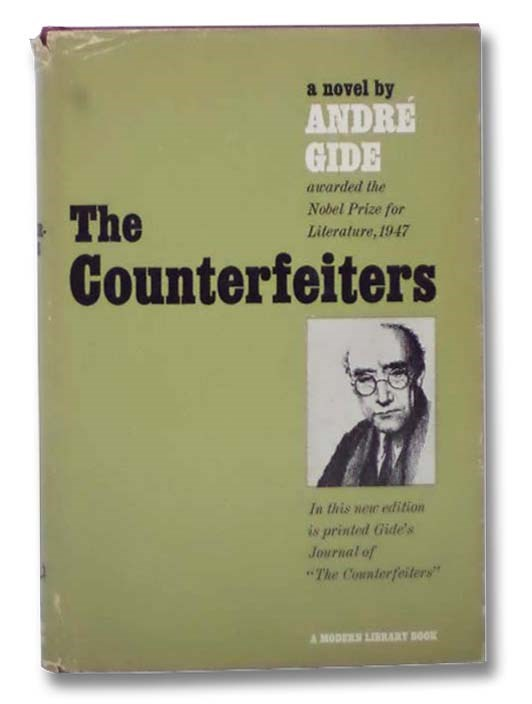
\includegraphics[max width=0.95\textwidth,
                        max height=0.58000\textheight]{{Images/counterfeiters}.jpg}
                \end{center}
            \end{column}
        \end{columns}
    }
\end{frame}
\begin{frame}[t]{Round 3 --- Famous Foreign-Language Literary Works --- \mbox{Answer 8}}
    \vspace{-0.5em}
    \begin{block}{Question}
        \emph{Der Proce{\ss}}
    \end{block}

    \visible<2->{
        \begin{columns}[T,totalwidth=\linewidth]
            \begin{column}{0.32\linewidth}
                \begin{block}{Answer}
                    \emph{The Trial} (Franz Kafka)
                \end{block}
            \end{column}
            \begin{column}{0.65\linewidth}
                \begin{center}
                    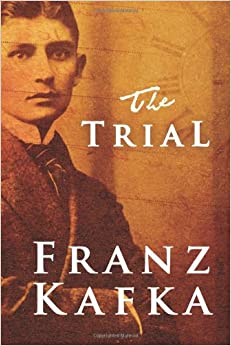
\includegraphics[max width=0.95\textwidth,
                        max height=0.58000\textheight]{{Images/thetrial}.jpg}
                \end{center}
            \end{column}
        \end{columns}
    }
\end{frame}
\begin{frame}[t]{Round 3 --- Famous Foreign-Language Literary Works --- \mbox{Answer 9}}
    \vspace{-0.5em}
    \begin{block}{Question}
        \emph{La condition humaine}
    \end{block}

    \visible<2->{
        \begin{columns}[T,totalwidth=\linewidth]
            \begin{column}{0.32\linewidth}
                \begin{block}{Answer}
                    \emph{Man's Fate} / \emph{Storm in Shanghai} / \emph{Man's Estate} (Malraux)
                \end{block}
            \end{column}
            \begin{column}{0.65\linewidth}
                \begin{center}
                    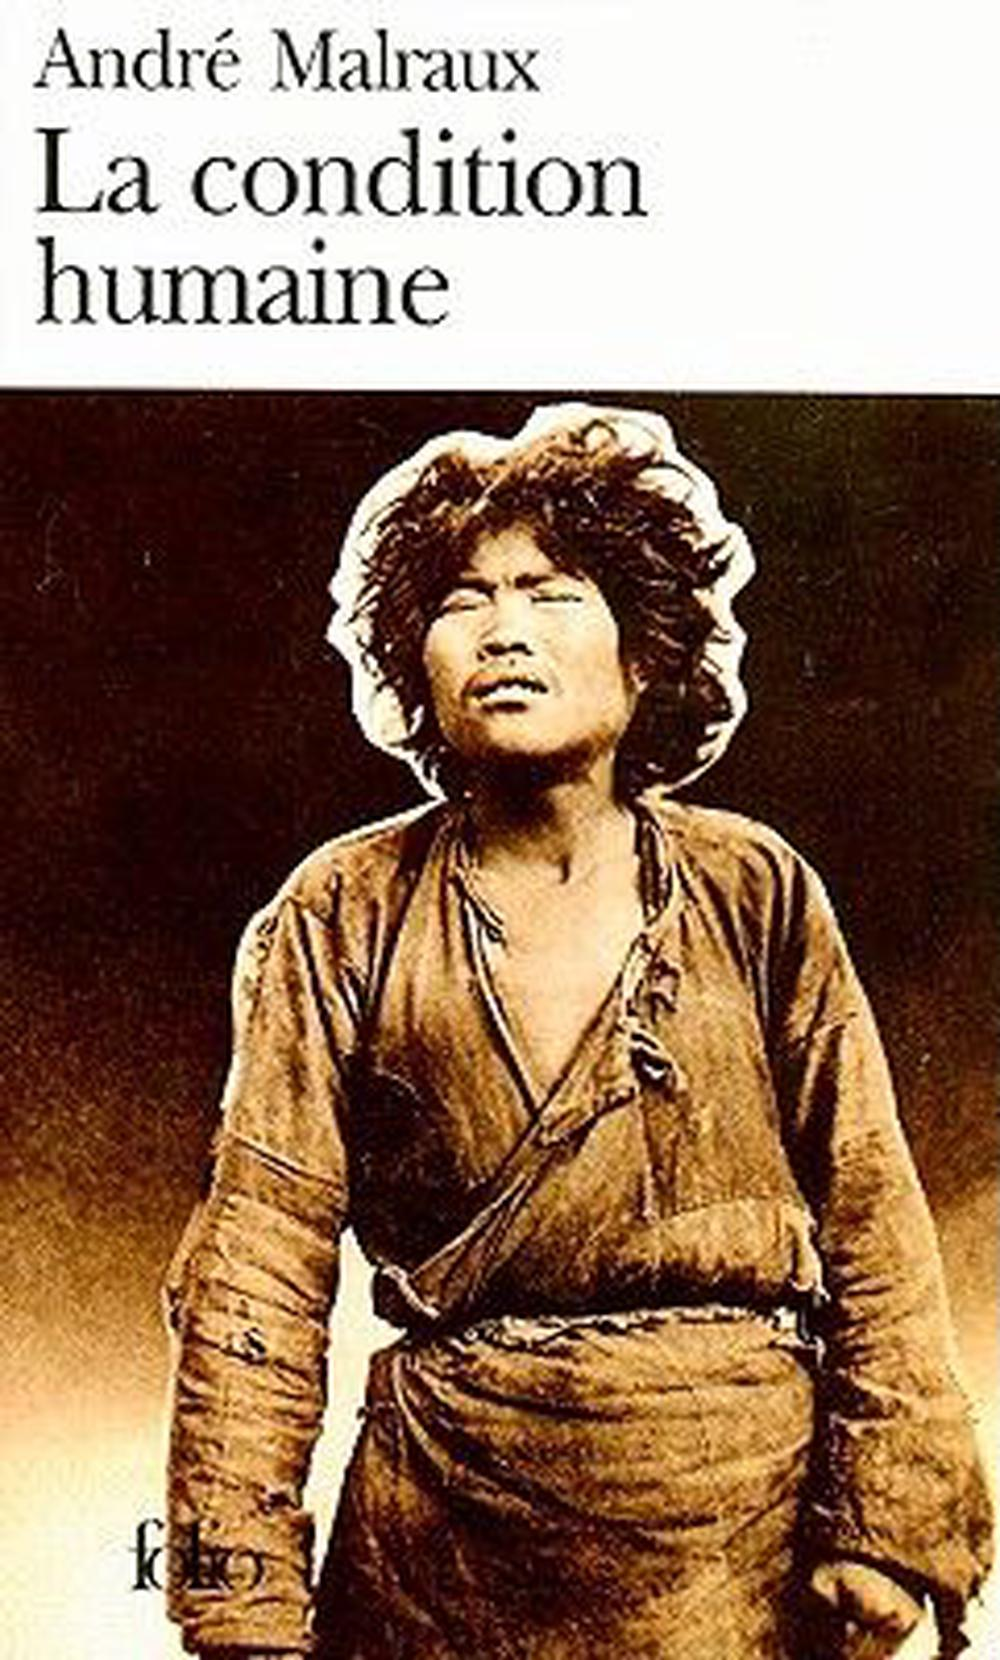
\includegraphics[max width=0.95\textwidth,
                        max height=0.58000\textheight]{{Images/mansfate}.jpg}
                \end{center}
            \end{column}
        \end{columns}
    }
\end{frame}
\begin{frame}[t]{Round 3 --- Famous Foreign-Language Literary Works --- \mbox{Answer 10}}
    \vspace{-0.5em}
    \begin{block}{Question}
        \emph{Sei personaggi in cerca d'autore}
    \end{block}

    \visible<2->{
        \begin{columns}[T,totalwidth=\linewidth]
            \begin{column}{0.32\linewidth}
                \begin{block}{Answer}
                    \emph{Six Characters in Search of an Author} (Pirandello)
                \end{block}
            \end{column}
            \begin{column}{0.65\linewidth}
                \begin{center}
                    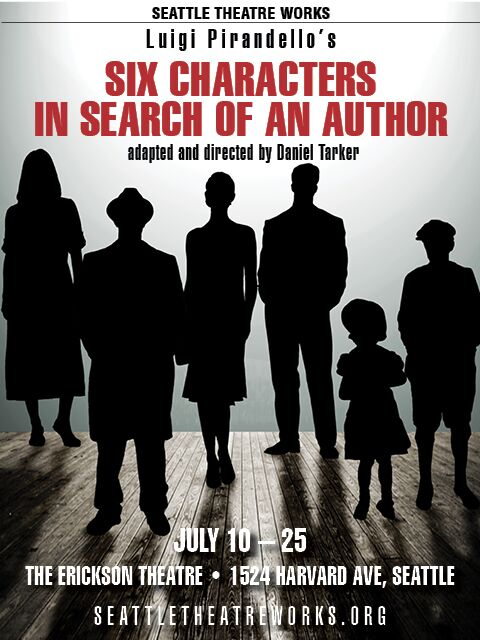
\includegraphics[max width=0.95\textwidth,
                        max height=0.58000\textheight]{{Images/sixcharacters}.jpg}
                \end{center}
            \end{column}
        \end{columns}
    }
\end{frame}
\def\thisSectionName{Newspapers and Magazines}
\section{Round 4}
\subsection*{Q1}
\begin{frame}[t]{Round 4 --- Newspapers and Magazines --- \mbox{Question 1}}
    \vspace{-0.5em}
    \begin{columns}[T,totalwidth=\linewidth]
        \begin{column}{0.32\linewidth}
            \begin{block}{Question}
                In the famous photo shown here, which newspaper is Truman holding up?
            \end{block}
        \end{column}
        \begin{column}{0.65\linewidth}
            \begin{center}
                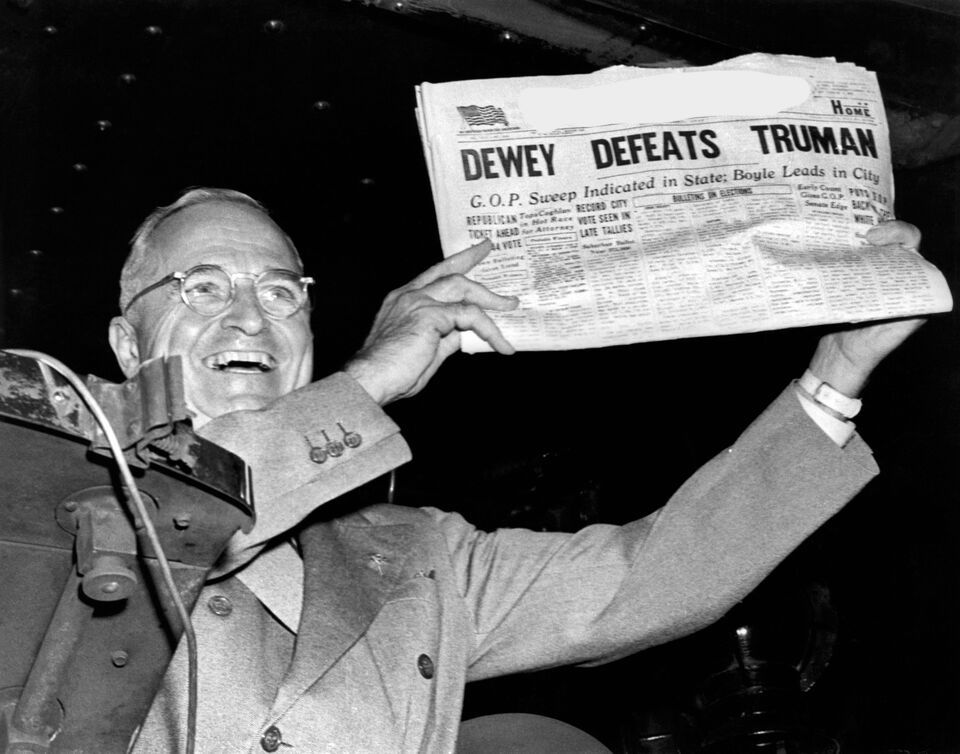
\includegraphics[max width=0.95\textwidth,max height=0.7\textheight]{{Images/DeweyTruman}.jpg}
            \end{center}
        \end{column}
    \end{columns}
\end{frame}
\subsection*{Q2}
\begin{frame}[t]{Round 4 --- Newspapers and Magazines --- \mbox{Question 2}}
    \vspace{-0.5em}
    \begin{block}{Question}
        Which newspaper's slogan is ``All the News That's Fit to Print''?
    \end{block}
\end{frame}
\subsection*{Q3}
\begin{frame}[t]{Round 4 --- Newspapers and Magazines --- \mbox{Question 3}}
    \vspace{-0.5em}
    \begin{columns}[T,totalwidth=\linewidth]
        \begin{column}{0.32\linewidth}
            \begin{block}{Question}
                What is the name of \emph{The New Yorker}'s mascot, pictured here, who is often seen peering at a butterfly through a monocle?
            \end{block}
        \end{column}
        \begin{column}{0.65\linewidth}
            \begin{center}
                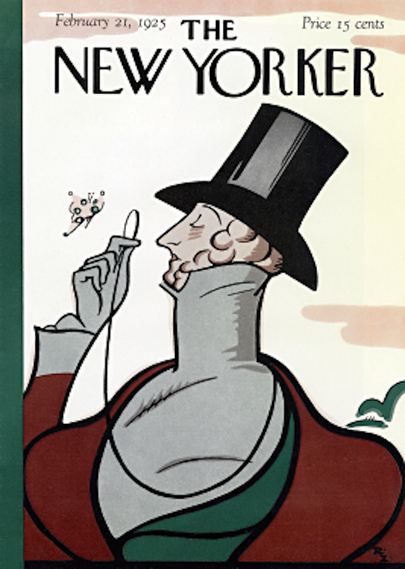
\includegraphics[max width=0.95\textwidth,max height=0.7\textheight]{{Images/eusticetilley}.jpg}
            \end{center}
        \end{column}
    \end{columns}
\end{frame}
\subsection*{Q4}
\begin{frame}[t]{Round 4 --- Newspapers and Magazines --- \mbox{Question 4}}
    \vspace{-0.5em}
    \begin{block}{Question}
        In a newspaper, what is the term for the line of text containing the name of an article's author?
    \end{block}
\end{frame}
\subsection*{Q5}
\begin{frame}[t]{Round 4 --- Newspapers and Magazines --- \mbox{Question 5}}
    \vspace{-0.5em}
    \begin{columns}[T,totalwidth=\linewidth]
        \begin{column}{0.32\linewidth}
            \begin{block}{Question}
                Which publication is known in part for its satirical and exaggerated cartoons, such as the one pictured here, that poke fun at the very nature of commentary cartoons?
            \end{block}
        \end{column}
        \begin{column}{0.65\linewidth}
            \begin{center}
                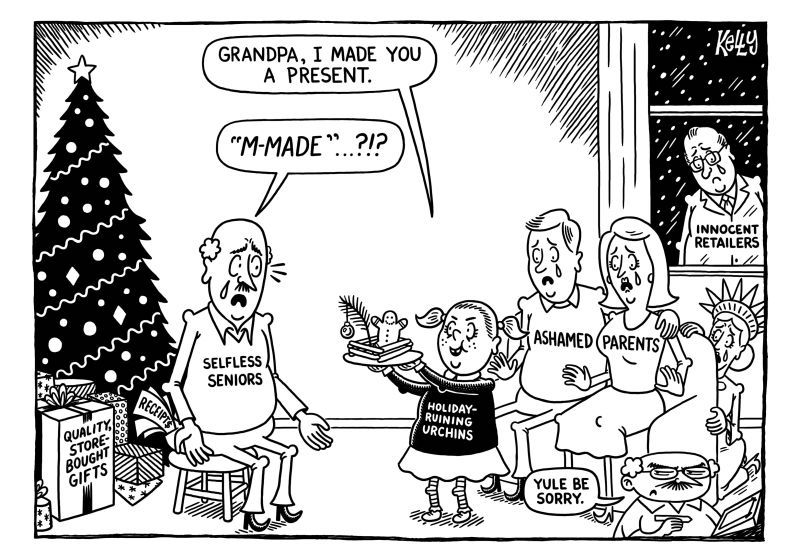
\includegraphics[max width=0.95\textwidth,max height=0.7\textheight]{{Images/onioncartoon}.jpg}
            \end{center}
        \end{column}
    \end{columns}
\end{frame}
\subsection*{Q6}
\begin{frame}[t]{Round 4 --- Newspapers and Magazines --- \mbox{Question 6}}
    \vspace{-0.5em}
    \begin{block}{Question}
        What is the name of the feature on the inside of the back cover of nearly every issue of \emph{Mad} magazine since 1964?
    \end{block}
\end{frame}
\subsection*{Q7}
\begin{frame}[t]{Round 4 --- Newspapers and Magazines --- \mbox{Question 7}}
    \vspace{-0.5em}
    \begin{block}{Question}
        Name either of the two Canadian newspapers that are nearly tied for being the most widely circulated newspaper in Canada.
    \end{block}
\end{frame}
\subsection*{Q8}
\begin{frame}[t]{Round 4 --- Newspapers and Magazines --- \mbox{Question 8}}
    \vspace{-0.5em}
    \begin{block}{Question}
        On which magazine's February 1982 cover were the pyramids of Giza altered, resulting in the first major scandal of the digital photography age?
    \end{block}
\end{frame}
\subsection*{Q9}
\begin{frame}[t]{Round 4 --- Newspapers and Magazines --- \mbox{Question 9}}
    \vspace{-0.5em}
    \begin{block}{Question}
        What is ``op-ed'' short for?
    \end{block}
\end{frame}
\subsection*{Q10}
\begin{frame}[t]{Round 4 --- Newspapers and Magazines --- \mbox{Question 10}}
    \vspace{-0.5em}
    \begin{block}{Question}
        Around the turn of the 20\textsuperscript{th} century, competition for readership between the newspapers the \emph{New York Journal} and the \emph{New York World} was fierce. Name the publisher of either newspaper.
    \end{block}
\end{frame}
\subsection{Answers}
\begin{frame}[t]{Round 4 --- Newspapers and Magazines --- \mbox{Answer 1}}
    \vspace{-0.5em}
    \begin{columns}[T,totalwidth=\linewidth]
        \begin{column}{0.32\linewidth}
            \begin{block}{Question}
                In the famous photo shown here, which newspaper is Truman holding up?
            \end{block}
            \visible<2->{
                \begin{block}{Answer}
                    \emph{The Chicago Tribune}
                \end{block}
            }
        \end{column}
        \begin{column}{0.65\linewidth}
            \begin{center}
                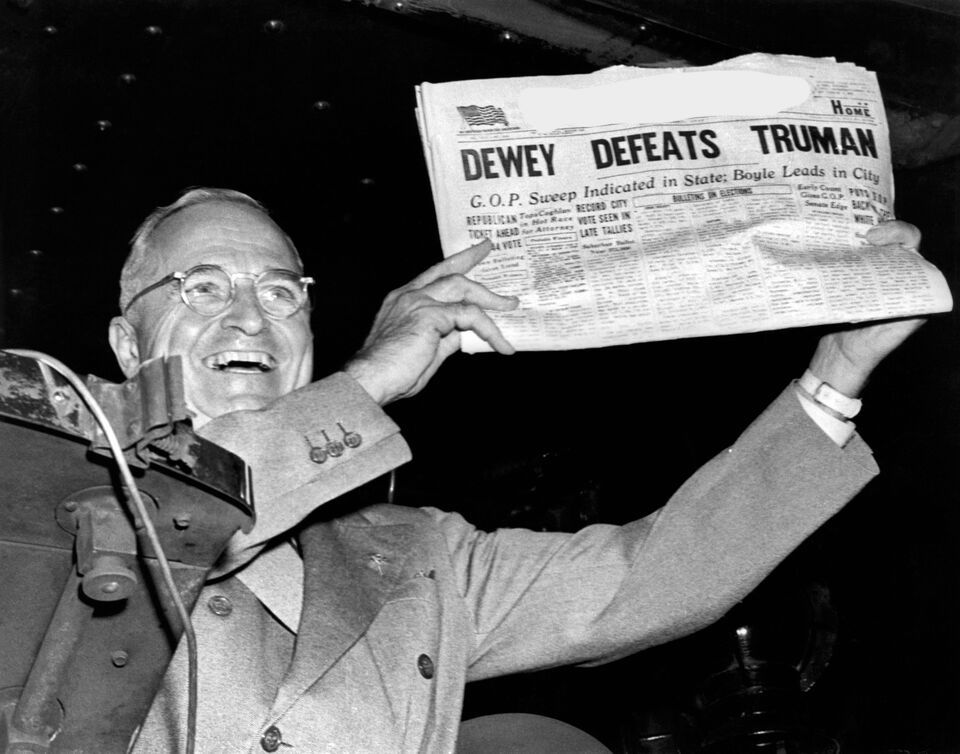
\includegraphics[max width=0.95\textwidth,max height=0.7\textheight]{{Images/DeweyTruman}.jpg}
            \end{center}
        \end{column}
    \end{columns}
\end{frame}
\begin{frame}[t]{Round 4 --- Newspapers and Magazines --- \mbox{Answer 2}}
    \vspace{-0.5em}
    \begin{block}{Question}
        Which newspaper's slogan is ``All the News That's Fit to Print''?
    \end{block}
    \visible<2->{
        \begin{block}{Answer}
            \emph{The New York Times}
        \end{block}
    }
\end{frame}
\begin{frame}[t]{Round 4 --- Newspapers and Magazines --- \mbox{Answer 3}}
    \vspace{-0.5em}
    \begin{columns}[T,totalwidth=\linewidth]
        \begin{column}{0.32\linewidth}
            \begin{block}{Question}
                What is the name of \emph{The New Yorker}'s mascot, pictured here, who is often seen peering at a butterfly through a monocle?
            \end{block}
            \visible<2->{
                \begin{block}{Answer}
                    Eustace Tilley
                \end{block}
            }
        \end{column}
        \begin{column}{0.65\linewidth}
            \begin{center}
                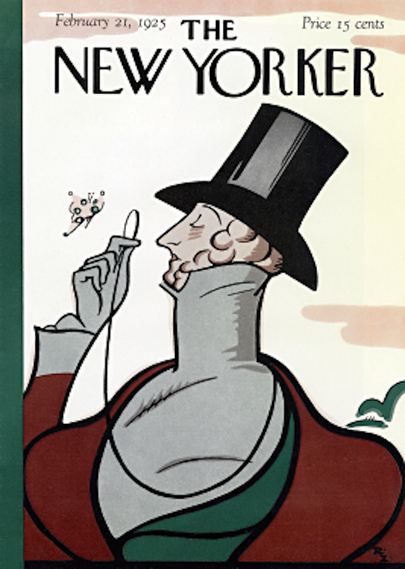
\includegraphics[max width=0.95\textwidth,max height=0.7\textheight]{{Images/eusticetilley}.jpg}
            \end{center}
        \end{column}
    \end{columns}
\end{frame}
\begin{frame}[t]{Round 4 --- Newspapers and Magazines --- \mbox{Answer 4}}
    \vspace{-0.5em}
    \begin{block}{Question}
        In a newspaper, what is the term for the line of text containing the name of an article's author?
    \end{block}
    \visible<2->{
        \begin{block}{Answer}
            The byline
        \end{block}
    }
\end{frame}
\begin{frame}[t]{Round 4 --- Newspapers and Magazines --- \mbox{Answer 5}}
    \vspace{-0.5em}
    \begin{columns}[T,totalwidth=\linewidth]
        \begin{column}{0.32\linewidth}
            \begin{block}{Question}
                Which publication is known in part for its satirical and exaggerated cartoons, such as the one pictured here, that poke fun at the very nature of commentary cartoons?
            \end{block}
            \visible<2->{
                \begin{block}{Answer}
                    \emph{The Onion}
                \end{block}
            }
        \end{column}
        \begin{column}{0.65\linewidth}
            \begin{center}
                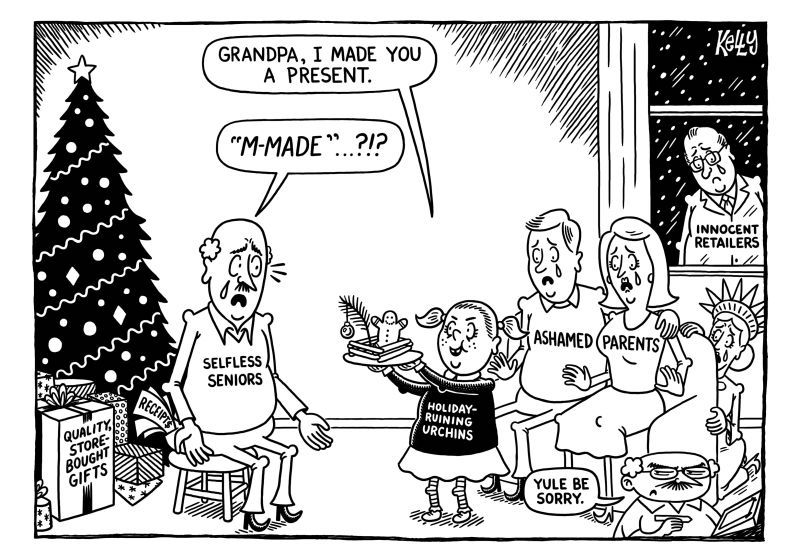
\includegraphics[max width=0.95\textwidth,max height=0.7\textheight]{{Images/onioncartoon}.jpg}
            \end{center}
        \end{column}
    \end{columns}
\end{frame}
\begin{frame}[t]{Round 4 --- Newspapers and Magazines --- \mbox{Answer 6}}
    \vspace{-0.5em}
    \begin{block}{Question}
        What is the name of the feature on the inside of the back cover of nearly every issue of \emph{Mad} magazine since 1964?
    \end{block}

    \visible<2->{
        \begin{columns}[T,totalwidth=\linewidth]
            \begin{column}{0.32\linewidth}
                \begin{block}{Answer}
                    The Fold-In
                \end{block}
            \end{column}
            \begin{column}{0.65\linewidth}
                \begin{center}
                    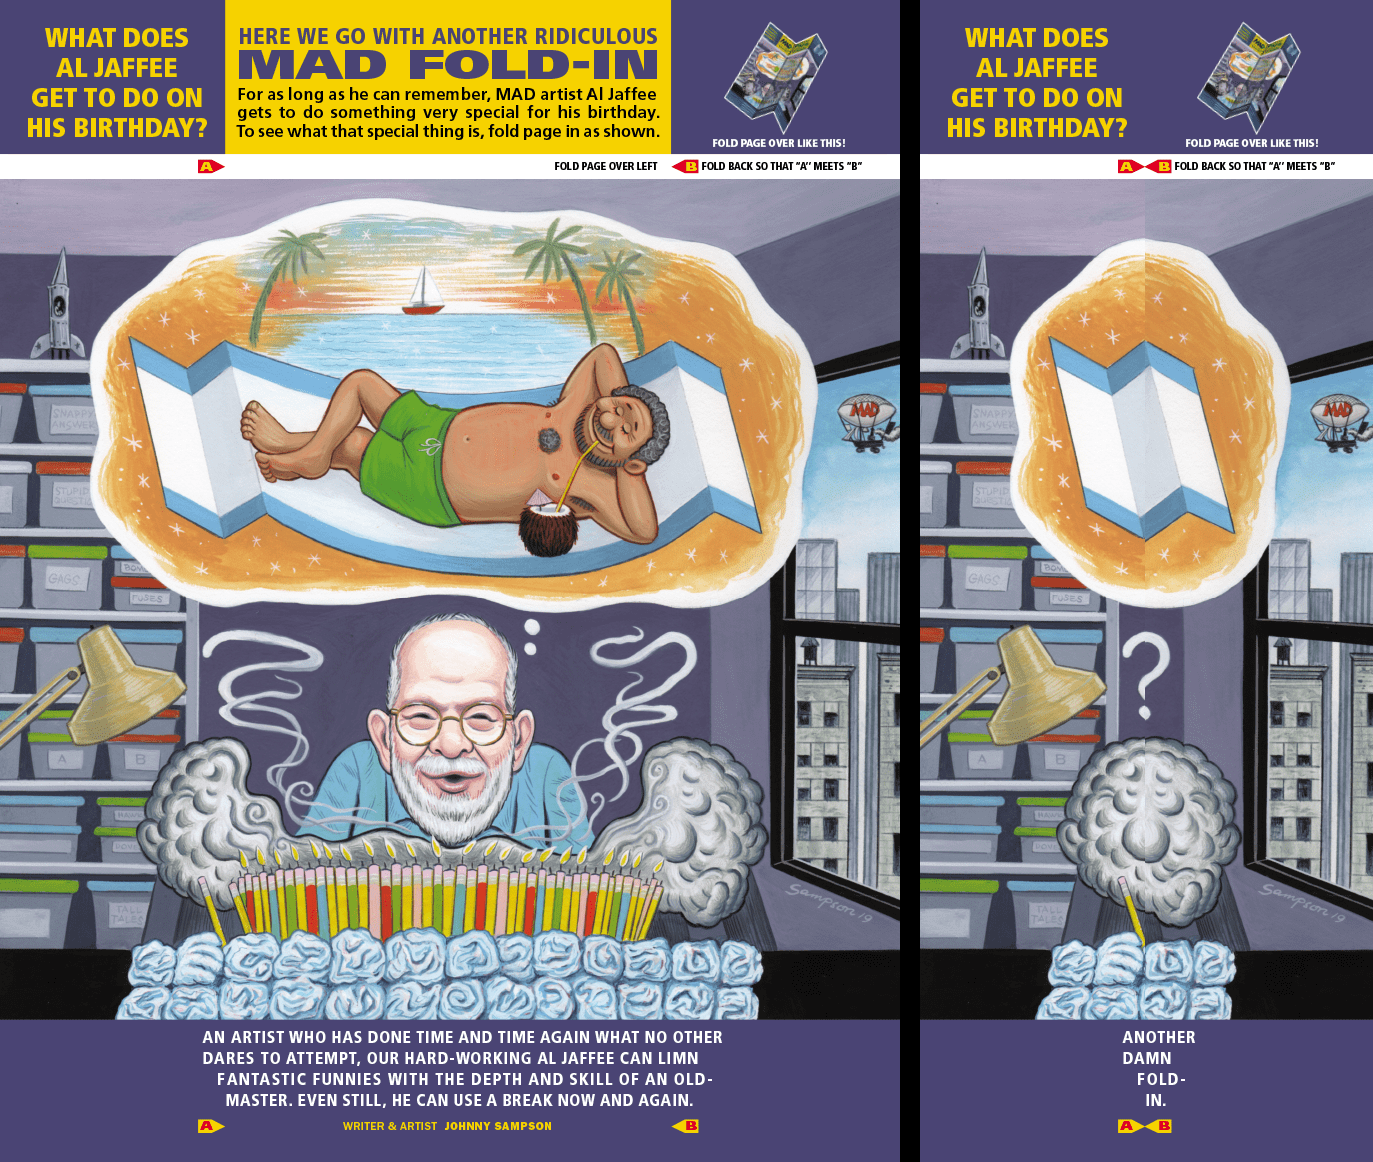
\includegraphics[max width=0.95\textwidth,
                        max height=0.48000\textheight]{{Images/foldin}.png}
                \end{center}
            \end{column}
        \end{columns}
    }
\end{frame}
\begin{frame}[t]{Round 4 --- Newspapers and Magazines --- \mbox{Answer 7}}
    \vspace{-0.5em}
    \begin{block}{Question}
        Name either of the two Canadian newspapers that are nearly tied for being the most widely circulated newspaper in Canada.
    \end{block}

    \visible<2->{
        \begin{columns}[T,totalwidth=\linewidth]
            \begin{column}{0.32\linewidth}
                \begin{block}{Answer}
                    \emph{The Globe and Mail} and the \emph{Toronto Star} (you only needed one)
                \end{block}
            \end{column}
            \begin{column}{0.65\linewidth}
                \begin{center}
                    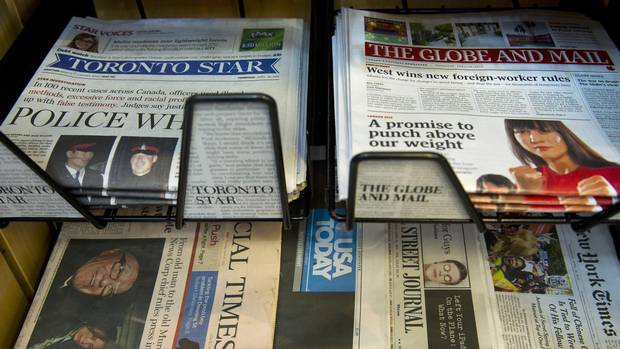
\includegraphics[max width=0.95\textwidth,
                        max height=0.48000\textheight]{{Images/canadianpaper}.JPG}
                \end{center}
            \end{column}
        \end{columns}
    }
\end{frame}
\begin{frame}[t]{Round 4 --- Newspapers and Magazines --- \mbox{Answer 8}}
    \vspace{-0.5em}
    \begin{block}{Question}
        On which magazine's February 1982 cover were the pyramids of Giza altered, resulting in the first major scandal of the digital photography age?
    \end{block}

    \visible<2->{
        \begin{columns}[T,totalwidth=\linewidth]
            \begin{column}{0.32\linewidth}
                \begin{block}{Answer}
                    \emph{National Geographic}
                \end{block}
            \end{column}
            \begin{column}{0.65\linewidth}
                \begin{center}
                    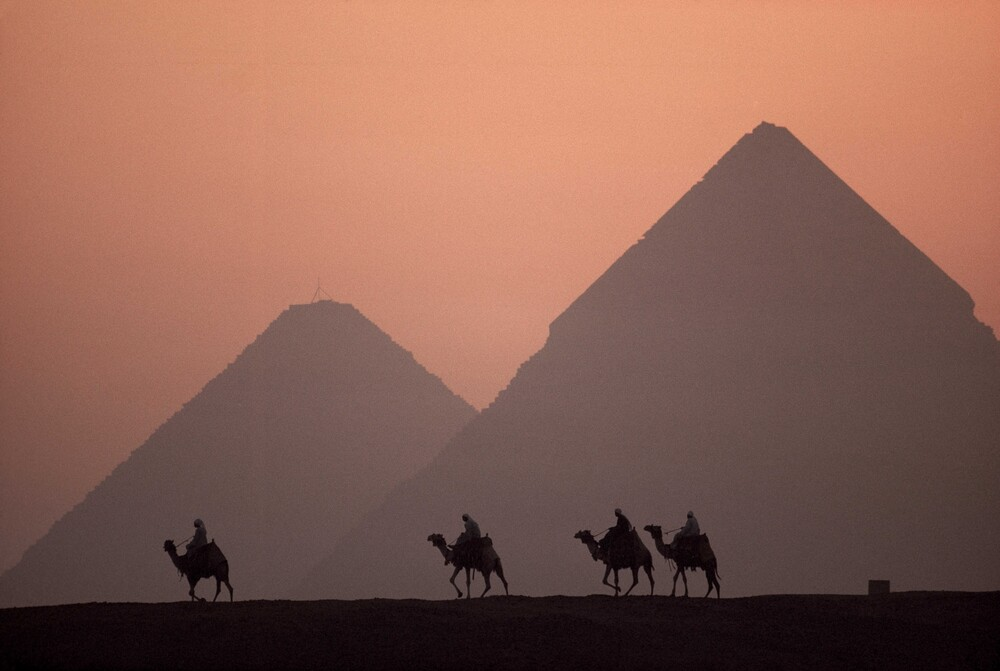
\includegraphics[max width=0.95\textwidth,
                        max height=0.48000\textheight]{{Images/pyramid}.jpg}
                \end{center}
            \end{column}
        \end{columns}
    }
\end{frame}
\begin{frame}[t]{Round 4 --- Newspapers and Magazines --- \mbox{Answer 9}}
    \vspace{-0.5em}
    \begin{block}{Question}
        What is ``op-ed'' short for?
    \end{block}

    \visible<2->{
        \begin{columns}[T,totalwidth=\linewidth]
            \begin{column}{0.32\linewidth}
                \begin{block}{Answer}
                    ``Opposite the editorial page'' (\emph{not} opinions and editorials)
                \end{block}
            \end{column}
            \begin{column}{0.65\linewidth}
                \begin{center}
                    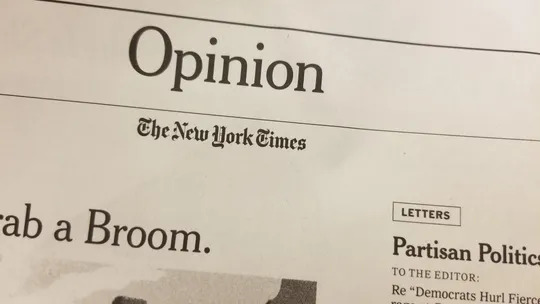
\includegraphics[max width=0.95\textwidth,
                        max height=0.58000\textheight]{{Images/oped}.jpg}
                \end{center}
            \end{column}
        \end{columns}
    }
\end{frame}
\begin{frame}[t]{Round 4 --- Newspapers and Magazines --- \mbox{Answer 10}}
    \vspace{-0.5em}
    \begin{block}{Question}
        Around the turn of the 20\textsuperscript{th} century, competition for readership between the newspapers the \emph{New York Journal} and the \emph{New York World} was fierce. Name the publisher of either newspaper.
    \end{block}

    \visible<2->{
        \begin{columns}[T,totalwidth=\linewidth]
            \begin{column}{0.32\linewidth}
                \begin{block}{Answer}
                    William Randolph Hearst and Joseph Pulitzer (the \emph{Journal} and the \emph{World}, respectively; we only needed one)
                \end{block}
            \end{column}
            \begin{column}{0.65\linewidth}
                \begin{center}
                    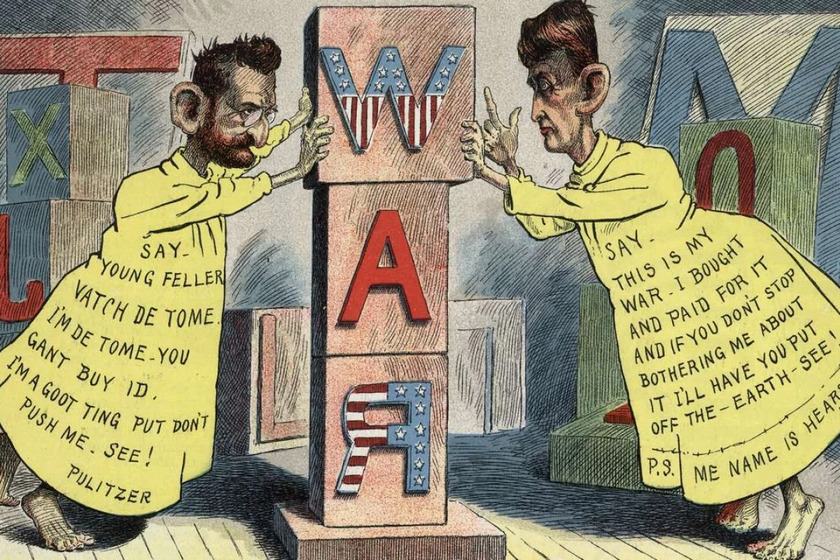
\includegraphics[max width=0.95\textwidth,
                        max height=0.38000\textheight]{{Images/yellowjournalism}.jpg}
                \end{center}
            \end{column}
        \end{columns}
    }
\end{frame}
\def\thisSectionName{One of the things this city is famous for is\ldots}
\section{Round 5}
\subsection*{Q1}
\begin{frame}[t]{Round 5 --- One of the things this city is famous for is\ldots --- \mbox{Question 1}}
    \vspace{-0.5em}
    \begin{block}{Question}
        The Mouth of Truth
    \end{block}
\end{frame}
\subsection*{Q2}
\begin{frame}[t]{Round 5 --- One of the things this city is famous for is\ldots --- \mbox{Question 2}}
    \vspace{-0.5em}
    \begin{block}{Question}
        The Gateway Arch
    \end{block}
\end{frame}
\subsection*{Q3}
\begin{frame}[t]{Round 5 --- One of the things this city is famous for is\ldots --- \mbox{Question 3}}
    \vspace{-0.5em}
    \begin{block}{Question}
        The Coit Tower
    \end{block}
\end{frame}
\subsection*{Q4}
\begin{frame}[t]{Round 5 --- One of the things this city is famous for is\ldots --- \mbox{Question 4}}
    \vspace{-0.5em}
    \begin{block}{Question}
        The Bund
    \end{block}
\end{frame}
\subsection*{Q5}
\begin{frame}[t]{Round 5 --- One of the things this city is famous for is\ldots --- \mbox{Question 5}}
    \vspace{-0.5em}
    \begin{block}{Question}
        Promenade des Anglais
    \end{block}
\end{frame}
\subsection*{Q6}
\begin{frame}[t]{Round 5 --- One of the things this city is famous for is\ldots --- \mbox{Question 6}}
    \vspace{-0.5em}
    \begin{block}{Question}
        Leonardo's painting of the Last Supper
    \end{block}
\end{frame}
\subsection*{Q7}
\begin{frame}[t]{Round 5 --- One of the things this city is famous for is\ldots --- \mbox{Question 7}}
    \vspace{-0.5em}
    \begin{block}{Question}
        The terracotta warriors
    \end{block}
\end{frame}
\subsection*{Q8}
\begin{frame}[t]{Round 5 --- One of the things this city is famous for is\ldots --- \mbox{Question 8}}
    \vspace{-0.5em}
    \begin{block}{Question}
        The Rose Bowl
    \end{block}
\end{frame}
\subsection*{Q9}
\begin{frame}[t]{Round 5 --- One of the things this city is famous for is\ldots --- \mbox{Question 9}}
    \vspace{-0.5em}
    \begin{block}{Question}
        The cathedral that Monet painted again and again
    \end{block}
\end{frame}
\subsection*{Q10}
\begin{frame}[t]{Round 5 --- One of the things this city is famous for is\ldots --- \mbox{Question 10}}
    \vspace{-0.5em}
    \begin{block}{Question}
        Rosa Parks' refusal to move to the back of the bus
    \end{block}
\end{frame}
\subsection{Answers}
\begin{frame}[t]{Round 5 --- One of the things this city is famous for is\ldots --- \mbox{Answer 1}}
    \vspace{-0.5em}
    \begin{block}{Question}
        The Mouth of Truth
    \end{block}

    \visible<2->{
        \begin{columns}[T,totalwidth=\linewidth]
            \begin{column}{0.32\linewidth}
                \begin{block}{Answer}
                    Rome, Italy
                \end{block}
            \end{column}
            \begin{column}{0.65\linewidth}
                \begin{center}
                    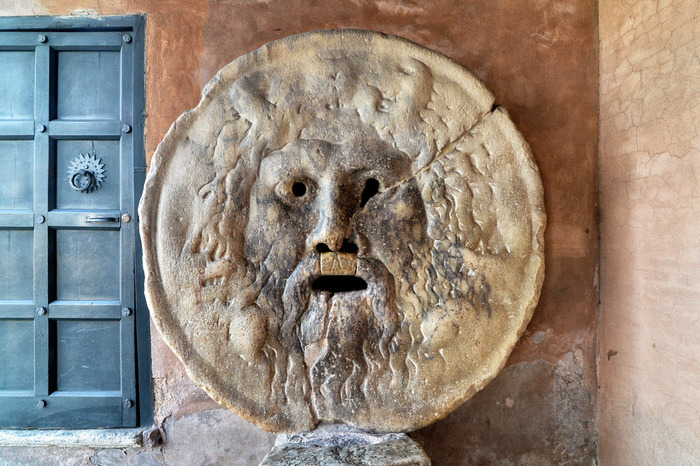
\includegraphics[max width=0.95\textwidth,
                        max height=0.58000\textheight]{{Images/mouthoftruth}.jpg}
                \end{center}
            \end{column}
        \end{columns}
    }
\end{frame}
\begin{frame}[t]{Round 5 --- One of the things this city is famous for is\ldots --- \mbox{Answer 2}}
    \vspace{-0.5em}
    \begin{block}{Question}
        The Gateway Arch
    \end{block}

    \visible<2->{
        \begin{columns}[T,totalwidth=\linewidth]
            \begin{column}{0.32\linewidth}
                \begin{block}{Answer}
                    St.\ Louis, Missouri
                \end{block}
            \end{column}
            \begin{column}{0.65\linewidth}
                \begin{center}
                    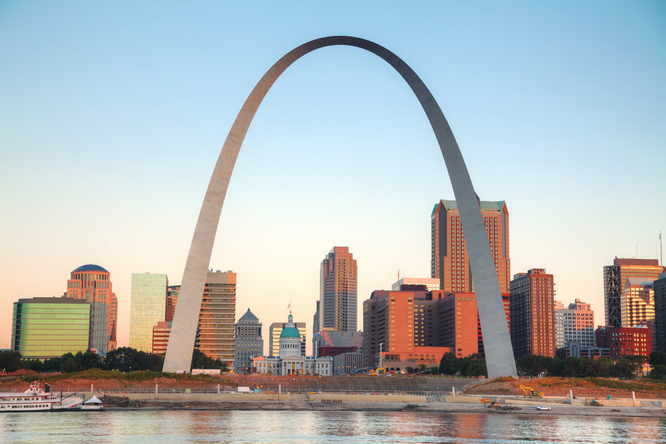
\includegraphics[max width=0.95\textwidth,
                        max height=0.58000\textheight]{{Images/stlarch}.jpg}
                \end{center}
            \end{column}
        \end{columns}
    }
\end{frame}
\begin{frame}[t]{Round 5 --- One of the things this city is famous for is\ldots --- \mbox{Answer 3}}
    \vspace{-0.5em}
    \begin{block}{Question}
        The Coit Tower
    \end{block}

    \visible<2->{
        \begin{columns}[T,totalwidth=\linewidth]
            \begin{column}{0.32\linewidth}
                \begin{block}{Answer}
                    San Francisco, California
                \end{block}
            \end{column}
            \begin{column}{0.65\linewidth}
                \begin{center}
                    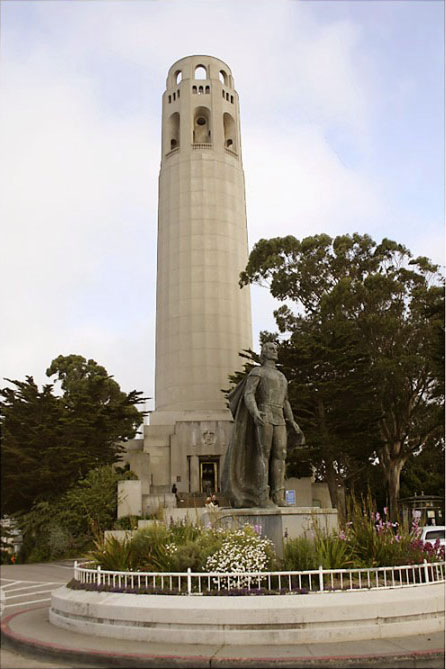
\includegraphics[max width=0.95\textwidth,
                        max height=0.58000\textheight]{{Images/Coittower1}.jpg}
                \end{center}
            \end{column}
        \end{columns}
    }
\end{frame}
\begin{frame}[t]{Round 5 --- One of the things this city is famous for is\ldots --- \mbox{Answer 4}}
    \vspace{-0.5em}
    \begin{block}{Question}
        The Bund
    \end{block}

    \visible<2->{
        \begin{columns}[T,totalwidth=\linewidth]
            \begin{column}{0.32\linewidth}
                \begin{block}{Answer}
                    Shanghai, China
                \end{block}
            \end{column}
            \begin{column}{0.65\linewidth}
                \begin{center}
                    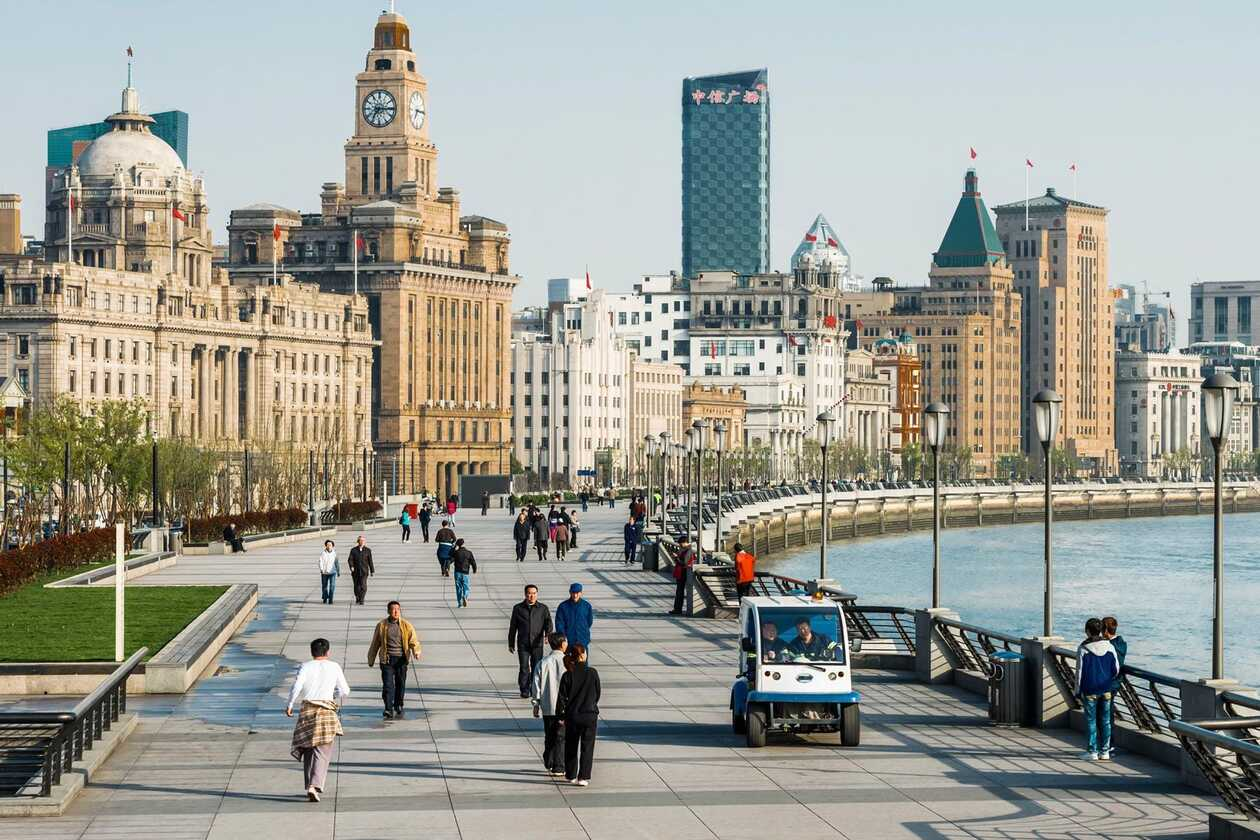
\includegraphics[max width=0.95\textwidth,
                        max height=0.58000\textheight]{{Images/bund}.jpg}
                \end{center}
            \end{column}
        \end{columns}
    }
\end{frame}
\begin{frame}[t]{Round 5 --- One of the things this city is famous for is\ldots --- \mbox{Answer 5}}
    \vspace{-0.5em}
    \begin{block}{Question}
        Promenade des Anglais
    \end{block}

    \visible<2->{
        \begin{columns}[T,totalwidth=\linewidth]
            \begin{column}{0.32\linewidth}
                \begin{block}{Answer}
                    Nice, France
                \end{block}
            \end{column}
            \begin{column}{0.65\linewidth}
                \begin{center}
                    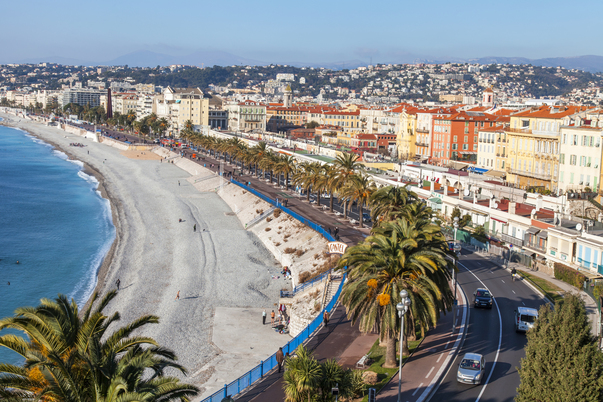
\includegraphics[max width=0.95\textwidth,
                        max height=0.58000\textheight]{{Images/anglais}.jpg}
                \end{center}
            \end{column}
        \end{columns}
    }
\end{frame}
\begin{frame}[t]{Round 5 --- One of the things this city is famous for is\ldots --- \mbox{Answer 6}}
    \vspace{-0.5em}
    \begin{block}{Question}
        Leonardo's painting of the Last Supper
    \end{block}

    \visible<2->{
        \begin{columns}[T,totalwidth=\linewidth]
            \begin{column}{0.32\linewidth}
                \begin{block}{Answer}
                    Milan, Italy
                \end{block}
            \end{column}
            \begin{column}{0.65\linewidth}
                \begin{center}
                    \includegraphics[max width=0.95\textwidth,
                        max height=0.58000\textheight]{{Images/lastsupper}.jpg}
                \end{center}
            \end{column}
        \end{columns}
    }
\end{frame}
\begin{frame}[t]{Round 5 --- One of the things this city is famous for is\ldots --- \mbox{Answer 7}}
    \vspace{-0.5em}
    \begin{block}{Question}
        The terracotta warriors
    \end{block}

    \visible<2->{
        \begin{columns}[T,totalwidth=\linewidth]
            \begin{column}{0.32\linewidth}
                \begin{block}{Answer}
                    Xian, China
                \end{block}
            \end{column}
            \begin{column}{0.65\linewidth}
                \begin{center}
                    \includegraphics[max width=0.95\textwidth,
                        max height=0.58000\textheight]{{Images/tcw}.jpg}
                \end{center}
            \end{column}
        \end{columns}
    }
\end{frame}
\begin{frame}[t]{Round 5 --- One of the things this city is famous for is\ldots --- \mbox{Answer 8}}
    \vspace{-0.5em}
    \begin{block}{Question}
        The Rose Bowl
    \end{block}

    \visible<2->{
        \begin{columns}[T,totalwidth=\linewidth]
            \begin{column}{0.32\linewidth}
                \begin{block}{Answer}
                    Pasadena, California
                \end{block}
            \end{column}
            \begin{column}{0.65\linewidth}
                \begin{center}
                    \includegraphics[max width=0.95\textwidth,
                        max height=0.58000\textheight]{{Images/rosebowl}.jpg}
                \end{center}
            \end{column}
        \end{columns}
    }
\end{frame}
\begin{frame}[t]{Round 5 --- One of the things this city is famous for is\ldots --- \mbox{Answer 9}}
    \vspace{-0.5em}
    \begin{block}{Question}
        The cathedral that Monet painted again and again
    \end{block}

    \visible<2->{
        \begin{columns}[T,totalwidth=\linewidth]
            \begin{column}{0.32\linewidth}
                \begin{block}{Answer}
                    Rouen, France
                \end{block}
            \end{column}
            \begin{column}{0.65\linewidth}
                \begin{center}
                    \includegraphics[max width=0.95\textwidth,
                        max height=0.58000\textheight]{{Images/monet}.jpg}
                \end{center}
            \end{column}
        \end{columns}
    }
\end{frame}
\begin{frame}[t]{Round 5 --- One of the things this city is famous for is\ldots --- \mbox{Answer 10}}
    \vspace{-0.5em}
    \begin{block}{Question}
        Rosa Parks' refusal to move to the back of the bus
    \end{block}

    \visible<2->{
        \begin{columns}[T,totalwidth=\linewidth]
            \begin{column}{0.32\linewidth}
                \begin{block}{Answer}
                    Montgomery, Alabama
                \end{block}
            \end{column}
            \begin{column}{0.65\linewidth}
                \begin{center}
                    \includegraphics[max width=0.95\textwidth,
                        max height=0.58000\textheight]{{Images/rosaparks}.jpeg}
                \end{center}
            \end{column}
        \end{columns}
    }
\end{frame}
\def\thisSectionName{Winter Sports}
\section{Round 6}
\subsection*{Q1}
\begin{frame}[t]{Round 6 --- Winter Sports --- \mbox{Question 1}}
    \vspace{-0.5em}
    \begin{block}{Question}
        Which winter sport was originally called ``snurfing''?
    \end{block}
\end{frame}
\subsection*{Q2}
\begin{frame}[t]{Round 6 --- Winter Sports --- \mbox{Question 2}}
    \vspace{-0.5em}
    \begin{block}{Question}
        If a figure skater completes a triple axel, how many degrees will they have rotated?
    \end{block}
\end{frame}
\subsection*{Q3}
\begin{frame}[t]{Round 6 --- Winter Sports --- \mbox{Question 3}}
    \vspace{-0.5em}
    \begin{block}{Question}
        Which two sports comprise the biathlon?
    \end{block}
\end{frame}
\subsection*{Q4}
\begin{frame}[t]{Round 6 --- Winter Sports --- \mbox{Question 4}}
    \vspace{-0.5em}
    \begin{block}{Question}
        What is a piste (which rhymes with ``east'')?
    \end{block}
\end{frame}
\subsection*{Q5}
\begin{frame}[t]{Round 6 --- Winter Sports --- \mbox{Question 5}}
    \vspace{-0.5em}
    \begin{block}{Question}
        Name any one of the three  cities in the world that have hosted the Winter Olympics twice.
    \end{block}
\end{frame}
\subsection*{Q6}
\begin{frame}[t]{Round 6 --- Winter Sports --- \mbox{Question 6}}
    \vspace{-0.5em}
    \begin{block}{Question}
        To within two, how many rounds was the longest shootout in NHL history?
    \end{block}
\end{frame}
\subsection*{Q7}
\begin{frame}[t]{Round 6 --- Winter Sports --- \mbox{Question 7}}
    \vspace{-0.5em}
    \begin{block}{Question}
        Which saint, who spent four decades doing missionary work in the Alps, is the patron saint of skiing, snowboarding, and mountaineering?
    \end{block}
\end{frame}
\subsection*{Q8}
\begin{frame}[t]{Round 6 --- Winter Sports --- \mbox{Question 8}}
    \vspace{-0.5em}
    \begin{block}{Question}
        In doubles luge, how do the two teammates lie on the luge? We need: whether they lie face up or face down, feet first or head first, and how the two athletes are positioned relative to each other.
    \end{block}
\end{frame}
\subsection*{Q9}
\begin{frame}[t]{Round 6 --- Winter Sports --- \mbox{Question 9}}
    \vspace{-0.5em}
    \begin{block}{Question}
        The French \emph{marche} became which English word that is used as a command in a winter sport?
    \end{block}
\end{frame}
\subsection*{Q10}
\begin{frame}[t]{Round 6 --- Winter Sports --- \mbox{Question 10}}
    \vspace{-0.5em}
    \begin{block}{Question}
        In curling, what is the name of the central circle --- curling's equivalent of the bullseye --- that competitors try to get their stones near?
    \end{block}
\end{frame}
\subsection{Answers}
\begin{frame}[t]{Round 6 --- Winter Sports --- \mbox{Answer 1}}
    \vspace{-0.5em}
    \begin{block}{Question}
        Which winter sport was originally called ``snurfing''?
    \end{block}

    \visible<2->{
        \begin{columns}[T,totalwidth=\linewidth]
            \begin{column}{0.32\linewidth}
                \begin{block}{Answer}
                    Snowboarding (a portmanteau of ``snow'' and ``surfing'')
                \end{block}
            \end{column}
            \begin{column}{0.65\linewidth}
                \begin{center}
                    \includegraphics[max width=0.95\textwidth,
                        max height=0.53000\textheight]{{Images/snurf}.jpg}
                \end{center}
            \end{column}
        \end{columns}
    }
\end{frame}
\begin{frame}[t]{Round 6 --- Winter Sports --- \mbox{Answer 2}}
    \vspace{-0.5em}
    \begin{block}{Question}
        If a figure skater completes a triple axel, how many degrees will they have rotated?
    \end{block}

    \visible<2->{
        \begin{columns}[T,totalwidth=\linewidth]
            \begin{column}{0.32\linewidth}
                \begin{block}{Answer}
                    \( 1260^\circ \) (a triple axel is three and a half turns, and \( 3.5\times 360^\circ=1260^\circ \))
                \end{block}
            \end{column}
            \begin{column}{0.65\linewidth}
                \begin{center}
                    \includegraphics[max width=0.95\textwidth,
                        max height=0.53000\textheight]{{Images/tripleaxel}.jpg}
                \end{center}
            \end{column}
        \end{columns}
    }
\end{frame}
\begin{frame}[t]{Round 6 --- Winter Sports --- \mbox{Answer 3}}
    \vspace{-0.5em}
    \begin{block}{Question}
        Which two sports comprise the biathlon?
    \end{block}

    \visible<2->{
        \begin{columns}[T,totalwidth=\linewidth]
            \begin{column}{0.32\linewidth}
                \begin{block}{Answer}
                    Cross-country skiing and rifle shooting (or just skiing and shooting; but you needed both)
                \end{block}
            \end{column}
            \begin{column}{0.65\linewidth}
                \begin{center}
                    \includegraphics[max width=0.95\textwidth,
                        max height=0.58000\textheight]{{Images/biathlon}.jpg}
                \end{center}
            \end{column}
        \end{columns}
    }
\end{frame}
\begin{frame}[t]{Round 6 --- Winter Sports --- \mbox{Answer 4}}
    \vspace{-0.5em}
    \begin{block}{Question}
        What is a piste (which rhymes with ``east'')?
    \end{block}

    \visible<2->{
        \begin{columns}[T,totalwidth=\linewidth]
            \begin{column}{0.32\linewidth}
                \begin{block}{Answer}
                    A groomed snowy path down a mountain for skiing or other winter mountain sports (we'll also accept ``ski run'', ``ski trail'', and ``what they go down during the Winter Olympics'')
                \end{block}
            \end{column}
            \begin{column}{0.65\linewidth}
                \begin{center}
                    \includegraphics[max width=0.95\textwidth,
                        max height=0.58000\textheight]{{Images/piste}.jpg}
                \end{center}
            \end{column}
        \end{columns}
    }
\end{frame}
\begin{frame}[t]{Round 6 --- Winter Sports --- \mbox{Answer 5}}
    \vspace{-0.5em}
    \begin{block}{Question}
        Name any one of the three  cities in the world that have hosted the Winter Olympics twice.
    \end{block}

    \visible<2->{
        \begin{columns}[T,totalwidth=\linewidth]
            \begin{column}{0.32\linewidth}
                \begin{block}{Answer}
                    Lake Placid, NY, Innsbruck, Austria, and  St.\ Moritz, Switzerland (you only needed one)
                \end{block}
            \end{column}
            \begin{column}{0.65\linewidth}
                \begin{center}
                    \includegraphics[max width=0.95\textwidth,
                        max height=0.53000\textheight]{{Images/placid}.jpg}
                \end{center}
            \end{column}
        \end{columns}
    }
\end{frame}
\begin{frame}[t]{Round 6 --- Winter Sports --- \mbox{Answer 6}}
    \vspace{-0.5em}
    \begin{block}{Question}
        To within two, how many rounds was the longest shootout in NHL history?
    \end{block}

    \visible<2->{
        \begin{columns}[T,totalwidth=\linewidth]
            \begin{column}{0.32\linewidth}
                \begin{block}{Answer}
                    Twenty (18--22 will be accepted)
                \end{block}
            \end{column}
            \begin{column}{0.65\linewidth}
                \begin{center}
                    \includegraphics[max width=0.95\textwidth,
                        max height=0.53000\textheight]{{Images/shootout}.jpg}
                \end{center}
            \end{column}
        \end{columns}
    }
\end{frame}
\begin{frame}[t]{Round 6 --- Winter Sports --- \mbox{Answer 7}}
    \vspace{-0.5em}
    \begin{block}{Question}
        Which saint, who spent four decades doing missionary work in the Alps, is the patron saint of skiing, snowboarding, and mountaineering?
    \end{block}

    \visible<2->{
        \begin{columns}[T,totalwidth=\linewidth]
            \begin{column}{0.32\linewidth}
                \begin{block}{Answer}
                    St.\ Bernard
                \end{block}
            \end{column}
            \begin{column}{0.65\linewidth}
                \begin{center}
                    \includegraphics[max width=0.95\textwidth,
                        max height=0.48000\textheight]{{Images/stbernard}.jpg}
                \end{center}
            \end{column}
        \end{columns}
    }
\end{frame}
\begin{frame}[t]{Round 6 --- Winter Sports --- \mbox{Answer 8}}
    \vspace{-0.5em}
    \begin{block}{Question}
        In doubles luge, how do the two teammates lie on the luge? We need: whether they lie face up or face down, feet first or head first, and how the two athletes are positioned relative to each other.
    \end{block}

    \visible<2->{
        \begin{columns}[T,totalwidth=\linewidth]
            \begin{column}{0.32\linewidth}
                \begin{block}{Answer}
                    On their backs, feet first, and one on top of the other
                \end{block}
            \end{column}
            \begin{column}{0.65\linewidth}
                \begin{center}
                    \includegraphics[max width=0.95\textwidth,
                        max height=0.43000\textheight]{{Images/luge}.jpg}
                \end{center}
            \end{column}
        \end{columns}
    }
\end{frame}
\begin{frame}[t]{Round 6 --- Winter Sports --- \mbox{Answer 9}}
    \vspace{-0.5em}
    \begin{block}{Question}
        The French \emph{marche} became which English word that is used as a command in a winter sport?
    \end{block}

    \visible<2->{
        \begin{columns}[T,totalwidth=\linewidth]
            \begin{column}{0.32\linewidth}
                \begin{block}{Answer}
                    Mush! (used in dog sledding)
                \end{block}
            \end{column}
            \begin{column}{0.65\linewidth}
                \begin{center}
                    \includegraphics[max width=0.95\textwidth,
                        max height=0.53000\textheight]{{Images/dogsled}.jpg}
                \end{center}
            \end{column}
        \end{columns}
    }
\end{frame}
\begin{frame}[t]{Round 6 --- Winter Sports --- \mbox{Answer 10}}
    \vspace{-0.5em}
    \begin{block}{Question}
        In curling, what is the name of the central circle --- curling's equivalent of the bullseye --- that competitors try to get their stones near?
    \end{block}

    \visible<2->{
        \begin{columns}[T,totalwidth=\linewidth]
            \begin{column}{0.32\linewidth}
                \begin{block}{Answer}
                    The button (we'll also accept ``pin'' and ``tee'', although they're technically the center of that circle)
                \end{block}
            \end{column}
            \begin{column}{0.65\linewidth}
                \begin{center}
                    \includegraphics[max width=0.95\textwidth,
                        max height=0.48000\textheight]{{Images/curling}.jpg}
                \end{center}
            \end{column}
        \end{columns}
    }
\end{frame}
\def\thisSectionName{Cartoons and the Funny Pages}
\section{Round 7}
\subsection*{Q1}
\begin{frame}[t]{Round 7 --- Cartoons and the Funny Pages --- \mbox{Question 1}}
    \vspace{-0.5em}
    \begin{block}{Question}
        What is the name of Popeye's nemesis?
    \end{block}
\end{frame}
\subsection*{Q2}
\begin{frame}[t]{Round 7 --- Cartoons and the Funny Pages --- \mbox{Question 2}}
    \vspace{-0.5em}
    \begin{block}{Question}
        In \emph{Dilbert}, what is the name of Dilbert's pet dog?
    \end{block}
\end{frame}
\subsection*{Q3}
\begin{frame}[t]{Round 7 --- Cartoons and the Funny Pages --- \mbox{Question 3}}
    \vspace{-0.5em}
    \begin{block}{Question}
        What Irish immigrant kid from New York's tenements was one of the first comic strip characters to appear in the color Sunday comics?
    \end{block}
\end{frame}
\subsection*{Q4}
\begin{frame}[t]{Round 7 --- Cartoons and the Funny Pages --- \mbox{Question 4}}
    \vspace{-0.5em}
    \begin{block}{Question}
        What 19\textsuperscript{th} Century  political cartoonist is generally credited with having produced the first modern image of the American Santa Claus?
    \end{block}
\end{frame}
\subsection*{Q5}
\begin{frame}[t]{Round 7 --- Cartoons and the Funny Pages --- \mbox{Question 5}}
    \vspace{-0.5em}
    \begin{block}{Question}
        What is the name of Charlie Brown's little sister?
    \end{block}
\end{frame}
\subsection*{Q6}
\begin{frame}[t]{Round 7 --- Cartoons and the Funny Pages --- \mbox{Question 6}}
    \vspace{-0.5em}
    \begin{block}{Question}
        What comic strip character put a spin on Admiral Perry's famous report that ``We have met the enemy and he is ours?''
    \end{block}
\end{frame}
\subsection*{Q7}
\begin{frame}[t]{Round 7 --- Cartoons and the Funny Pages --- \mbox{Question 7}}
    \vspace{-0.5em}
    \begin{block}{Question}
        Which comic strip about an African-American family became so popular that it was made into a TV show on Adult Swim?
    \end{block}
\end{frame}
\subsection*{Q8}
\begin{frame}[t]{Round 7 --- Cartoons and the Funny Pages --- \mbox{Question 8}}
    \vspace{-0.5em}
    \begin{block}{Question}
        What square-jawed police detective used a two-way wrist radio?
    \end{block}
\end{frame}
\subsection*{Q9}
\begin{frame}[t]{Round 7 --- Cartoons and the Funny Pages --- \mbox{Question 9}}
    \vspace{-0.5em}
    \begin{block}{Question}
        What comic strip character's heart was full of unrequited love for Ignatz Mouse? (Spelling counts.)
    \end{block}
\end{frame}
\subsection*{Q10}
\begin{frame}[t]{Round 7 --- Cartoons and the Funny Pages --- \mbox{Question 10}}
    \vspace{-0.5em}
    \begin{columns}[T,totalwidth=\linewidth]
        \begin{column}{0.32\linewidth}
            \begin{block}{Question}
                Who authored the cartoon shown here?
            \end{block}
        \end{column}
        \begin{column}{0.65\linewidth}
            \begin{center}
                \includegraphics[max width=0.95\textwidth,max height=0.7\textheight]{{Images/HairCutReminder}.jpg}
            \end{center}
        \end{column}
    \end{columns}
\end{frame}
\subsection{Answers}
\begin{frame}[t]{Round 7 --- Cartoons and the Funny Pages --- \mbox{Answer 1}}
    \vspace{-0.5em}
    \begin{block}{Question}
        What is the name of Popeye's nemesis?
    \end{block}

    \visible<2->{
        \begin{columns}[T,totalwidth=\linewidth]
            \begin{column}{0.32\linewidth}
                \begin{block}{Answer}
                    Bluto or Brutus
                \end{block}
            \end{column}
            \begin{column}{0.65\linewidth}
                \begin{center}
                    \includegraphics[max width=0.95\textwidth,
                        max height=0.58000\textheight]{{Images/Blutowindow}.jpg}
                \end{center}
            \end{column}
        \end{columns}
    }
\end{frame}
\begin{frame}[t]{Round 7 --- Cartoons and the Funny Pages --- \mbox{Answer 2}}
    \vspace{-0.5em}
    \begin{block}{Question}
        In \emph{Dilbert}, what is the name of Dilbert's pet dog?
    \end{block}

    \visible<2->{
        \begin{columns}[T,totalwidth=\linewidth]
            \begin{column}{0.32\linewidth}
                \begin{block}{Answer}
                    Dogbert
                \end{block}
            \end{column}
            \begin{column}{0.65\linewidth}
                \begin{center}
                    \includegraphics[max width=0.95\textwidth,
                        max height=0.53000\textheight]{{Images/dogbert}.png}
                \end{center}
            \end{column}
        \end{columns}
    }
\end{frame}
\begin{frame}[t]{Round 7 --- Cartoons and the Funny Pages --- \mbox{Answer 3}}
    \vspace{-0.5em}
    \begin{block}{Question}
        What Irish immigrant kid from New York's tenements was one of the first comic strip characters to appear in the color Sunday comics?
    \end{block}

    \visible<2->{
        \begin{columns}[T,totalwidth=\linewidth]
            \begin{column}{0.32\linewidth}
                \begin{block}{Answer}
                    The Yellow Kid
                \end{block}
            \end{column}
            \begin{column}{0.65\linewidth}
                \begin{center}
                    \includegraphics[max width=0.95\textwidth,
                        max height=0.48000\textheight]{{Images/yellowkid}.jpg}
                \end{center}
            \end{column}
        \end{columns}
    }
\end{frame}
\begin{frame}[t]{Round 7 --- Cartoons and the Funny Pages --- \mbox{Answer 4}}
    \vspace{-0.5em}
    \begin{block}{Question}
        What 19\textsuperscript{th} Century  political cartoonist is generally credited with having produced the first modern image of the American Santa Claus?
    \end{block}

    \visible<2->{
        \begin{columns}[T,totalwidth=\linewidth]
            \begin{column}{0.32\linewidth}
                \begin{block}{Answer}
                    Thomas Nast
                \end{block}
            \end{column}
            \begin{column}{0.65\linewidth}
                \begin{center}
                    \includegraphics[max width=0.95\textwidth,
                        max height=0.43000\textheight]{{Images/santanast}.jpg}
                \end{center}
            \end{column}
        \end{columns}
    }
\end{frame}
\begin{frame}[t]{Round 7 --- Cartoons and the Funny Pages --- \mbox{Answer 5}}
    \vspace{-0.5em}
    \begin{block}{Question}
        What is the name of Charlie Brown's little sister?
    \end{block}

    \visible<2->{
        \begin{columns}[T,totalwidth=\linewidth]
            \begin{column}{0.32\linewidth}
                \begin{block}{Answer}
                    Sally
                \end{block}
            \end{column}
            \begin{column}{0.65\linewidth}
                \begin{center}
                    \includegraphics[max width=0.95\textwidth,
                        max height=0.58000\textheight]{{Images/charliebrown}.jpg}
                \end{center}
            \end{column}
        \end{columns}
    }
\end{frame}
\begin{frame}[t]{Round 7 --- Cartoons and the Funny Pages --- \mbox{Answer 6}}
    \vspace{-0.5em}
    \begin{block}{Question}
        What comic strip character put a spin on Admiral Perry's famous report that ``We have met the enemy and he is ours?''
    \end{block}

    \visible<2->{
        \begin{columns}[T,totalwidth=\linewidth]
            \begin{column}{0.32\linewidth}
                \begin{block}{Answer}
                    Pogo (''We have met the enemy and he is us.'')
                \end{block}
            \end{column}
            \begin{column}{0.65\linewidth}
                \begin{center}
                    \includegraphics[max width=0.95\textwidth,
                        max height=0.48000\textheight]{{Images/pogo}.jpg}
                \end{center}
            \end{column}
        \end{columns}
    }
\end{frame}
\begin{frame}[t]{Round 7 --- Cartoons and the Funny Pages --- \mbox{Answer 7}}
    \vspace{-0.5em}
    \begin{block}{Question}
        Which comic strip about an African-American family became so popular that it was made into a TV show on Adult Swim?
    \end{block}

    \visible<2->{
        \begin{columns}[T,totalwidth=\linewidth]
            \begin{column}{0.32\linewidth}
                \begin{block}{Answer}
                    \emph{The Boondocks}
                \end{block}
            \end{column}
            \begin{column}{0.65\linewidth}
                \begin{center}
                    \includegraphics[max width=0.95\textwidth,
                        max height=0.48000\textheight]{{Images/boondocks}.jpg}
                \end{center}
            \end{column}
        \end{columns}
    }
\end{frame}
\begin{frame}[t]{Round 7 --- Cartoons and the Funny Pages --- \mbox{Answer 8}}
    \vspace{-0.5em}
    \begin{block}{Question}
        What square-jawed police detective used a two-way wrist radio?
    \end{block}

    \visible<2->{
        \begin{columns}[T,totalwidth=\linewidth]
            \begin{column}{0.32\linewidth}
                \begin{block}{Answer}
                    Dick Tracy
                \end{block}
            \end{column}
            \begin{column}{0.65\linewidth}
                \begin{center}
                    \includegraphics[max width=0.95\textwidth,
                        max height=0.53000\textheight]{{Images/dicktracy}.jpg}
                \end{center}
            \end{column}
        \end{columns}
    }
\end{frame}
\begin{frame}[t]{Round 7 --- Cartoons and the Funny Pages --- \mbox{Answer 9}}
    \vspace{-0.5em}
    \begin{block}{Question}
        What comic strip character's heart was full of unrequited love for Ignatz Mouse? (Spelling counts.)
    \end{block}

    \visible<2->{
        \begin{columns}[T,totalwidth=\linewidth]
            \begin{column}{0.32\linewidth}
                \begin{block}{Answer}
                    Krazy Kat
                \end{block}
            \end{column}
            \begin{column}{0.65\linewidth}
                \begin{center}
                    \includegraphics[max width=0.95\textwidth,
                        max height=0.53000\textheight]{{Images/krazykat}.jpg}
                \end{center}
            \end{column}
        \end{columns}
    }
\end{frame}
\begin{frame}[t]{Round 7 --- Cartoons and the Funny Pages --- \mbox{Answer 10}}
    \vspace{-0.5em}
    \begin{columns}[T,totalwidth=\linewidth]
        \begin{column}{0.32\linewidth}
            \begin{block}{Question}
                Who authored the cartoon shown here?
            \end{block}
            \visible<2->{
                \begin{block}{Answer}
                    Rube Goldberg
                \end{block}
            }
        \end{column}
        \begin{column}{0.65\linewidth}
            \begin{center}
                \includegraphics[max width=0.95\textwidth,max height=0.7\textheight]{{Images/HairCutReminder}.jpg}
            \end{center}
        \end{column}
    \end{columns}
\end{frame}
\def\thisSectionName{Specialized Words II}
\section{Round 8}
\subsection*{Q1}
\begin{frame}[t]{Round 8 --- Specialized Words II --- \mbox{Question 1}}
    \vspace{-0.5em}
    \begin{block}{Question}
        In the context of hardware (non-computer), what is a \emph{peen}?
    \end{block}
\end{frame}
\subsection*{Q2}
\begin{frame}[t]{Round 8 --- Specialized Words II --- \mbox{Question 2}}
    \vspace{-0.5em}
    \begin{block}{Question}
        In mathematics, what is a lemma?
    \end{block}
\end{frame}
\subsection*{Q3}
\begin{frame}[t]{Round 8 --- Specialized Words II --- \mbox{Question 3}}
    \vspace{-0.5em}
    \begin{block}{Question}
        What is an aglet?
    \end{block}
\end{frame}
\subsection*{Q4}
\begin{frame}[t]{Round 8 --- Specialized Words II --- \mbox{Question 4}}
    \vspace{-0.5em}
    \begin{block}{Question}
        In math and physics, what is the term for the direction perpendicular to a given surface?
    \end{block}
\end{frame}
\subsection*{Q5}
\begin{frame}[t]{Round 8 --- Specialized Words II --- \mbox{Question 5}}
    \vspace{-0.5em}
    \begin{block}{Question}
        Here's a topical one: what are fomites (pronounced ``foam-mitt-tees'')?
    \end{block}
\end{frame}
\subsection*{Q6}
\begin{frame}[t]{Round 8 --- Specialized Words II --- \mbox{Question 6}}
    \vspace{-0.5em}
    \begin{block}{Question}
        The ocular impairment ``amblyopia'' is better known by what colloquial name?
    \end{block}
\end{frame}
\subsection*{Q7}
\begin{frame}[t]{Round 8 --- Specialized Words II --- \mbox{Question 7}}
    \vspace{-0.5em}
    \begin{block}{Question}
        What is ``odontophobia'' the fear of?
    \end{block}
\end{frame}
\subsection*{Q8}
\begin{frame}[t]{Round 8 --- Specialized Words II --- \mbox{Question 8}}
    \vspace{-0.5em}
    \begin{block}{Question}
        What is a cheval mirror?
    \end{block}
\end{frame}
\subsection*{Q9}
\begin{frame}[t]{Round 8 --- Specialized Words II --- \mbox{Question 9}}
    \vspace{-0.5em}
    \begin{block}{Question}
        Which part of a horse does the \emph{withers} refer to?
    \end{block}
\end{frame}
\subsection*{Q10}
\begin{frame}[t]{Round 8 --- Specialized Words II --- \mbox{Question 10}}
    \vspace{-0.5em}
    \begin{block}{Question}
        In baseball, what is a \emph{battery}?
    \end{block}
\end{frame}
\subsection{Answers}
\begin{frame}[t]{Round 8 --- Specialized Words II --- \mbox{Answer 1}}
    \vspace{-0.5em}
    \begin{block}{Question}
        In the context of hardware (non-computer), what is a \emph{peen}?
    \end{block}

    \visible<2->{
        \begin{columns}[T,totalwidth=\linewidth]
            \begin{column}{0.32\linewidth}
                \begin{block}{Answer}
                    The side of a hammer's head opposite the face (e.g., the ball on a ball-peen hammer)
                \end{block}
            \end{column}
            \begin{column}{0.65\linewidth}
                \begin{center}
                    \includegraphics[max width=0.95\textwidth,
                        max height=0.53000\textheight]{{Images/ballpeenhammer}.jpg}
                \end{center}
            \end{column}
        \end{columns}
    }
\end{frame}
\begin{frame}[t]{Round 8 --- Specialized Words II --- \mbox{Answer 2}}
    \vspace{-0.5em}
    \begin{block}{Question}
        In mathematics, what is a lemma?
    \end{block}

    \visible<2->{
        \begin{columns}[T,totalwidth=\linewidth]
            \begin{column}{0.32\linewidth}
                \begin{block}{Answer}
                    A smaller theorem used to prove a larger result, or an ``auxiliary theorem''
                \end{block}
            \end{column}
            \begin{column}{0.65\linewidth}
                \begin{center}
                    \includegraphics[max width=0.95\textwidth,
                        max height=0.58000\textheight]{{Images/zorn}.jpg}
                \end{center}
            \end{column}
        \end{columns}
    }
\end{frame}
\begin{frame}[t]{Round 8 --- Specialized Words II --- \mbox{Answer 3}}
    \vspace{-0.5em}
    \begin{block}{Question}
        What is an aglet?
    \end{block}

    \visible<2->{
        \begin{columns}[T,totalwidth=\linewidth]
            \begin{column}{0.32\linewidth}
                \begin{block}{Answer}
                    The metal or plastic tube fixed tightly around each end of a shoelace
                \end{block}
            \end{column}
            \begin{column}{0.65\linewidth}
                \begin{center}
                    \includegraphics[max width=0.95\textwidth,
                        max height=0.58000\textheight]{{Images/aglet}.jpg}
                \end{center}
            \end{column}
        \end{columns}
    }
\end{frame}
\begin{frame}[t]{Round 8 --- Specialized Words II --- \mbox{Answer 4}}
    \vspace{-0.5em}
    \begin{block}{Question}
        In math and physics, what is the term for the direction perpendicular to a given surface?
    \end{block}

    \visible<2->{
        \begin{columns}[T,totalwidth=\linewidth]
            \begin{column}{0.32\linewidth}
                \begin{block}{Answer}
                    The normal
                \end{block}
            \end{column}
            \begin{column}{0.65\linewidth}
                \begin{center}
                    \includegraphics[max width=0.95\textwidth,
                        max height=0.53000\textheight]{{Images/normal}.jpg}
                \end{center}
            \end{column}
        \end{columns}
    }
\end{frame}
\begin{frame}[t]{Round 8 --- Specialized Words II --- \mbox{Answer 5}}
    \vspace{-0.5em}
    \begin{block}{Question}
        Here's a topical one: what are fomites (pronounced ``foam-mitt-tees'')?
    \end{block}

    \visible<2->{
        \begin{columns}[T,totalwidth=\linewidth]
            \begin{column}{0.32\linewidth}
                \begin{block}{Answer}
                    Surfaces that are likely to spread disease via contact
                \end{block}
            \end{column}
            \begin{column}{0.65\linewidth}
                \begin{center}
                    \includegraphics[max width=0.95\textwidth,
                        max height=0.53000\textheight]{{Images/fomite}.jpg}
                \end{center}
            \end{column}
        \end{columns}
    }
\end{frame}
\begin{frame}[t]{Round 8 --- Specialized Words II --- \mbox{Answer 6}}
    \vspace{-0.5em}
    \begin{block}{Question}
        The ocular impairment ``amblyopia'' is better known by what colloquial name?
    \end{block}

    \visible<2->{
        \begin{columns}[T,totalwidth=\linewidth]
            \begin{column}{0.32\linewidth}
                \begin{block}{Answer}
                    Lazy eye
                \end{block}
            \end{column}
            \begin{column}{0.65\linewidth}
                \begin{center}
                    \includegraphics[max width=0.95\textwidth,
                        max height=0.53000\textheight]{{Images/lazyeye}.jpg}
                \end{center}
            \end{column}
        \end{columns}
    }
\end{frame}
\begin{frame}[t]{Round 8 --- Specialized Words II --- \mbox{Answer 7}}
    \vspace{-0.5em}
    \begin{block}{Question}
        What is ``odontophobia'' the fear of?
    \end{block}

    \visible<2->{
        \begin{columns}[T,totalwidth=\linewidth]
            \begin{column}{0.32\linewidth}
                \begin{block}{Answer}
                    Dentists and / or dental procedures
                \end{block}
            \end{column}
            \begin{column}{0.65\linewidth}
                \begin{center}
                    \includegraphics[max width=0.95\textwidth,
                        max height=0.58000\textheight]{{Images/odontofobia}.jpg}
                \end{center}
            \end{column}
        \end{columns}
    }
\end{frame}
\begin{frame}[t]{Round 8 --- Specialized Words II --- \mbox{Answer 8}}
    \vspace{-0.5em}
    \begin{block}{Question}
        What is a cheval mirror?
    \end{block}

    \visible<2->{
        \begin{columns}[T,totalwidth=\linewidth]
            \begin{column}{0.32\linewidth}
                \begin{block}{Answer}
                    A full-length mirror on a hinge
                \end{block}
            \end{column}
            \begin{column}{0.65\linewidth}
                \begin{center}
                    \includegraphics[max width=0.95\textwidth,
                        max height=0.58000\textheight]{{Images/cheval}.jpg}
                \end{center}
            \end{column}
        \end{columns}
    }
\end{frame}
\begin{frame}[t]{Round 8 --- Specialized Words II --- \mbox{Answer 9}}
    \vspace{-0.5em}
    \begin{block}{Question}
        Which part of a horse does the \emph{withers} refer to?
    \end{block}

    \visible<2->{
        \begin{columns}[T,totalwidth=\linewidth]
            \begin{column}{0.32\linewidth}
                \begin{block}{Answer}
                    The highest part of its back / the base of the neck / above the shoulders / just below the mane
                \end{block}
            \end{column}
            \begin{column}{0.65\linewidth}
                \begin{center}
                    \includegraphics[max width=0.95\textwidth,
                        max height=0.53000\textheight]{{Images/Withers}.jpg}
                \end{center}
            \end{column}
        \end{columns}
    }
\end{frame}
\begin{frame}[t]{Round 8 --- Specialized Words II --- \mbox{Answer 10}}
    \vspace{-0.5em}
    \begin{block}{Question}
        In baseball, what is a \emph{battery}?
    \end{block}

    \visible<2->{
        \begin{columns}[T,totalwidth=\linewidth]
            \begin{column}{0.32\linewidth}
                \begin{block}{Answer}
                    A pitcher-catcher pair / the pitcher and catcher collectively
                \end{block}
            \end{column}
            \begin{column}{0.65\linewidth}
                \begin{center}
                    \includegraphics[max width=0.95\textwidth,
                        max height=0.58000\textheight]{{Images/marianojorge}.jpeg}
                \end{center}
            \end{column}
        \end{columns}
    }
\end{frame}
\def\thisSectionName{Other Things that Happened in 2020}
\section{Round 9}
\subsection*{Q1}
\begin{frame}[t]{Round 9 --- Other Things that Happened in 2020 --- \mbox{Question 1}}
    \vspace{-0.5em}
    \begin{block}{Question}
        What caused the Australian state of New South Wales to declare an emergency in January?
    \end{block}
\end{frame}
\subsection*{Q2}
\begin{frame}[t]{Round 9 --- Other Things that Happened in 2020 --- \mbox{Question 2}}
    \vspace{-0.5em}
    \begin{block}{Question}
        Which British royals decided to step away from the royal family?
    \end{block}
\end{frame}
\subsection*{Q3}
\begin{frame}[t]{Round 9 --- Other Things that Happened in 2020 --- \mbox{Question 3}}
    \vspace{-0.5em}
    \begin{block}{Question}
        On which website were the accounts of Barack Obama, Elon Musk, Bill Gates, and several other prominent people hacked in order to share Bitcoin scams?
    \end{block}
\end{frame}
\subsection*{Q4}
\begin{frame}[t]{Round 9 --- Other Things that Happened in 2020 --- \mbox{Question 4}}
    \vspace{-0.5em}
    \begin{block}{Question}
        What port city suffered a devastating explosion on August 4\textsuperscript{th}?
    \end{block}
\end{frame}
\subsection*{Q5}
\begin{frame}[t]{Round 9 --- Other Things that Happened in 2020 --- \mbox{Question 5}}
    \vspace{-0.5em}
    \begin{block}{Question}
        The price of what commodity briefly dropped below \$0 in April of this year? (Suppliers were paying people to take it off their hands.)
    \end{block}
\end{frame}
\subsection*{Q6}
\begin{frame}[t]{Round 9 --- Other Things that Happened in 2020 --- \mbox{Question 6}}
    \vspace{-0.5em}
    \begin{block}{Question}
        Which country --- in an environmentally sensitive but perhaps ill-timed gesture --- made public transportation free in February?
    \end{block}
\end{frame}
\subsection*{Q7}
\begin{frame}[t]{Round 9 --- Other Things that Happened in 2020 --- \mbox{Question 7}}
    \vspace{-0.5em}
    \begin{block}{Question}
        In May, which country became the first Central American country to legalize same-sex marriage?
    \end{block}
\end{frame}
\subsection*{Q8}
\begin{frame}[t]{Round 9 --- Other Things that Happened in 2020 --- \mbox{Question 8}}
    \vspace{-0.5em}
    \begin{block}{Question}
        Which film swept the Academy Awards?
    \end{block}
\end{frame}
\subsection*{Q9}
\begin{frame}[t]{Round 9 --- Other Things that Happened in 2020 --- \mbox{Question 9}}
    \vspace{-0.5em}
    \begin{block}{Question}
        This Asian head of state disappeared for while, leading to speculation that he was gravely ill or had died.
    \end{block}
\end{frame}
\subsection*{Q10}
\begin{frame}[t]{Round 9 --- Other Things that Happened in 2020 --- \mbox{Question 10}}
    \vspace{-0.5em}
    \begin{block}{Question}
        Which rock guitarist --- the leader of his eponymous band --- died on October 6\textsuperscript{th}\,?
    \end{block}
\end{frame}
\subsection{Answers}
\begin{frame}[t]{Round 9 --- Other Things that Happened in 2020 --- \mbox{Answer 1}}
    \vspace{-0.5em}
    \begin{block}{Question}
        What caused the Australian state of New South Wales to declare an emergency in January?
    \end{block}

    \visible<2->{
        \begin{columns}[T,totalwidth=\linewidth]
            \begin{column}{0.32\linewidth}
                \begin{block}{Answer}
                    Wildfires
                \end{block}
            \end{column}
            \begin{column}{0.65\linewidth}
                \begin{center}
                    \includegraphics[max width=0.95\textwidth,
                        max height=0.53000\textheight]{{Images/wildfire}.jpg}
                \end{center}
            \end{column}
        \end{columns}
    }
\end{frame}
\begin{frame}[t]{Round 9 --- Other Things that Happened in 2020 --- \mbox{Answer 2}}
    \vspace{-0.5em}
    \begin{block}{Question}
        Which British royals decided to step away from the royal family?
    \end{block}

    \visible<2->{
        \begin{columns}[T,totalwidth=\linewidth]
            \begin{column}{0.32\linewidth}
                \begin{block}{Answer}
                    The Duke and Duchess of Sussex --- Harry and Meghan
                \end{block}
            \end{column}
            \begin{column}{0.65\linewidth}
                \begin{center}
                    \includegraphics[max width=0.95\textwidth,
                        max height=0.53000\textheight]{{Images/markle}.jpg}
                \end{center}
            \end{column}
        \end{columns}
    }
\end{frame}
\begin{frame}[t]{Round 9 --- Other Things that Happened in 2020 --- \mbox{Answer 3}}
    \vspace{-0.5em}
    \begin{block}{Question}
        On which website were the accounts of Barack Obama, Elon Musk, Bill Gates, and several other prominent people hacked in order to share Bitcoin scams?
    \end{block}

    \visible<2->{
        \begin{columns}[T,totalwidth=\linewidth]
            \begin{column}{0.32\linewidth}
                \begin{block}{Answer}
                    Twitter
                \end{block}
            \end{column}
            \begin{column}{0.65\linewidth}
                \begin{center}
                    \includegraphics[max width=0.95\textwidth,
                        max height=0.48000\textheight]{{Images/twitterhack}.jpg}
                \end{center}
            \end{column}
        \end{columns}
    }
\end{frame}
\begin{frame}[t]{Round 9 --- Other Things that Happened in 2020 --- \mbox{Answer 4}}
    \vspace{-0.5em}
    \begin{block}{Question}
        What port city suffered a devastating explosion on August 4\textsuperscript{th}?
    \end{block}

    \visible<2->{
        \begin{columns}[T,totalwidth=\linewidth]
            \begin{column}{0.32\linewidth}
                \begin{block}{Answer}
                    Beirut
                \end{block}
            \end{column}
            \begin{column}{0.65\linewidth}
                \begin{center}
                    \includegraphics[max width=0.95\textwidth,
                        max height=0.53000\textheight]{{Images/beirut}.jpg}
                \end{center}
            \end{column}
        \end{columns}
    }
\end{frame}
\begin{frame}[t]{Round 9 --- Other Things that Happened in 2020 --- \mbox{Answer 5}}
    \vspace{-0.5em}
    \begin{block}{Question}
        The price of what commodity briefly dropped below \$0 in April of this year? (Suppliers were paying people to take it off their hands.)
    \end{block}

    \visible<2->{
        \begin{columns}[T,totalwidth=\linewidth]
            \begin{column}{0.32\linewidth}
                \begin{block}{Answer}
                    (Crude) oil
                \end{block}
            \end{column}
            \begin{column}{0.65\linewidth}
                \begin{center}
                    \includegraphics[max width=0.95\textwidth,
                        max height=0.48000\textheight]{{Images/oilneg}.png}
                \end{center}
            \end{column}
        \end{columns}
    }
\end{frame}
\begin{frame}[t]{Round 9 --- Other Things that Happened in 2020 --- \mbox{Answer 6}}
    \vspace{-0.5em}
    \begin{block}{Question}
        Which country --- in an environmentally sensitive but perhaps ill-timed gesture --- made public transportation free in February?
    \end{block}

    \visible<2->{
        \begin{columns}[T,totalwidth=\linewidth]
            \begin{column}{0.32\linewidth}
                \begin{block}{Answer}
                    Luxembourg
                \end{block}
            \end{column}
            \begin{column}{0.65\linewidth}
                \begin{center}
                    \includegraphics[max width=0.95\textwidth,
                        max height=0.48000\textheight]{{Images/luxembourg}.jpg}
                \end{center}
            \end{column}
        \end{columns}
    }
\end{frame}
\begin{frame}[t]{Round 9 --- Other Things that Happened in 2020 --- \mbox{Answer 7}}
    \vspace{-0.5em}
    \begin{block}{Question}
        In May, which country became the first Central American country to legalize same-sex marriage?
    \end{block}

    \visible<2->{
        \begin{columns}[T,totalwidth=\linewidth]
            \begin{column}{0.32\linewidth}
                \begin{block}{Answer}
                    Costa Rica
                \end{block}
            \end{column}
            \begin{column}{0.65\linewidth}
                \begin{center}
                    \includegraphics[max width=0.95\textwidth,
                        max height=0.53000\textheight]{{Images/costarica}.jpg}
                \end{center}
            \end{column}
        \end{columns}
    }
\end{frame}
\begin{frame}[t]{Round 9 --- Other Things that Happened in 2020 --- \mbox{Answer 8}}
    \vspace{-0.5em}
    \begin{block}{Question}
        Which film swept the Academy Awards?
    \end{block}

    \visible<2->{
        \begin{columns}[T,totalwidth=\linewidth]
            \begin{column}{0.32\linewidth}
                \begin{block}{Answer}
                    \emph{Parasite}
                \end{block}
            \end{column}
            \begin{column}{0.65\linewidth}
                \begin{center}
                    \includegraphics[max width=0.95\textwidth,
                        max height=0.58000\textheight]{{Images/parasite}.jpg}
                \end{center}
            \end{column}
        \end{columns}
    }
\end{frame}
\begin{frame}[t]{Round 9 --- Other Things that Happened in 2020 --- \mbox{Answer 9}}
    \vspace{-0.5em}
    \begin{block}{Question}
        This Asian head of state disappeared for while, leading to speculation that he was gravely ill or had died.
    \end{block}

    \visible<2->{
        \begin{columns}[T,totalwidth=\linewidth]
            \begin{column}{0.32\linewidth}
                \begin{block}{Answer}
                    Kim Jong-un
                \end{block}
            \end{column}
            \begin{column}{0.65\linewidth}
                \begin{center}
                    \includegraphics[max width=0.95\textwidth,
                        max height=0.48000\textheight]{{Images/kim}.jpg}
                \end{center}
            \end{column}
        \end{columns}
    }
\end{frame}
\begin{frame}[t]{Round 9 --- Other Things that Happened in 2020 --- \mbox{Answer 10}}
    \vspace{-0.5em}
    \begin{block}{Question}
        Which rock guitarist --- the leader of his eponymous band --- died on October 6\textsuperscript{th}\,?
    \end{block}

    \visible<2->{
        \begin{columns}[T,totalwidth=\linewidth]
            \begin{column}{0.32\linewidth}
                \begin{block}{Answer}
                    Eddie Van Halen
                \end{block}
            \end{column}
            \begin{column}{0.65\linewidth}
                \begin{center}
                    \includegraphics[max width=0.95\textwidth,
                        max height=0.48000\textheight]{{Images/vanhalen}.jpg}
                \end{center}
            \end{column}
        \end{columns}
    }
\end{frame}
\def\thisSectionName{Movies From Their Stills}
\section{Round 10}
\subsection*{Q1}
\begin{frame}[t]{Round 10 --- Movies From Their Stills --- \mbox{Question 1}}
    \vspace{-0.5em}
    \begin{columns}[T,totalwidth=\linewidth]
        \begin{column}{0.32\linewidth}
            \begin{block}{Question}
                Name the movie.
            \end{block}
        \end{column}
        \begin{column}{0.65\linewidth}
            \begin{center}
                \includegraphics[max width=0.95\textwidth,max height=0.7\textheight]{{Images/walter}.jpg}
            \end{center}
        \end{column}
    \end{columns}
\end{frame}
\subsection*{Q2}
\begin{frame}[t]{Round 10 --- Movies From Their Stills --- \mbox{Question 2}}
    \vspace{-0.5em}
    \begin{columns}[T,totalwidth=\linewidth]
        \begin{column}{0.32\linewidth}
            \begin{block}{Question}
                Name the movie.
            \end{block}
        \end{column}
        \begin{column}{0.65\linewidth}
            \begin{center}
                \includegraphics[max width=0.95\textwidth,max height=0.7\textheight]{{Images/grapesofwrath}.jpg}
            \end{center}
        \end{column}
    \end{columns}
\end{frame}
\subsection*{Q3}
\begin{frame}[t]{Round 10 --- Movies From Their Stills --- \mbox{Question 3}}
    \vspace{-0.5em}
    \begin{columns}[T,totalwidth=\linewidth]
        \begin{column}{0.32\linewidth}
            \begin{block}{Question}
                Name the movie.
            \end{block}
        \end{column}
        \begin{column}{0.65\linewidth}
            \begin{center}
                \includegraphics[max width=0.95\textwidth,max height=0.7\textheight]{{Images/seven-yearitch}.jpg}
            \end{center}
        \end{column}
    \end{columns}
\end{frame}
\subsection*{Q4}
\begin{frame}[t]{Round 10 --- Movies From Their Stills --- \mbox{Question 4}}
    \vspace{-0.5em}
    \begin{columns}[T,totalwidth=\linewidth]
        \begin{column}{0.32\linewidth}
            \begin{block}{Question}
                Name the movie.
            \end{block}
        \end{column}
        \begin{column}{0.65\linewidth}
            \begin{center}
                \includegraphics[max width=0.95\textwidth,max height=0.7\textheight]{{Images/bhc}.jpg}
            \end{center}
        \end{column}
    \end{columns}
\end{frame}
\subsection*{Q5}
\begin{frame}[t]{Round 10 --- Movies From Their Stills --- \mbox{Question 5}}
    \vspace{-0.5em}
    \begin{columns}[T,totalwidth=\linewidth]
        \begin{column}{0.32\linewidth}
            \begin{block}{Question}
                Name the movie.
            \end{block}
        \end{column}
        \begin{column}{0.65\linewidth}
            \begin{center}
                \includegraphics[max width=0.95\textwidth,max height=0.7\textheight]{{Images/taxidriver}.jpg}
            \end{center}
        \end{column}
    \end{columns}
\end{frame}
\subsection*{Q6}
\begin{frame}[t]{Round 10 --- Movies From Their Stills --- \mbox{Question 6}}
    \vspace{-0.5em}
    \begin{columns}[T,totalwidth=\linewidth]
        \begin{column}{0.32\linewidth}
            \begin{block}{Question}
                Name the movie.
            \end{block}
        \end{column}
        \begin{column}{0.65\linewidth}
            \begin{center}
                \includegraphics[max width=0.95\textwidth,max height=0.7\textheight]{{Images/inbruges}.jpg}
            \end{center}
        \end{column}
    \end{columns}
\end{frame}
\subsection*{Q7}
\begin{frame}[t]{Round 10 --- Movies From Their Stills --- \mbox{Question 7}}
    \vspace{-0.5em}
    \begin{columns}[T,totalwidth=\linewidth]
        \begin{column}{0.32\linewidth}
            \begin{block}{Question}
                Name the movie.
            \end{block}
        \end{column}
        \begin{column}{0.65\linewidth}
            \begin{center}
                \includegraphics[max width=0.95\textwidth,max height=0.7\textheight]{{Images/zoolander}.jpg}
            \end{center}
        \end{column}
    \end{columns}
\end{frame}
\subsection*{Q8}
\begin{frame}[t]{Round 10 --- Movies From Their Stills --- \mbox{Question 8}}
    \vspace{-0.5em}
    \begin{columns}[T,totalwidth=\linewidth]
        \begin{column}{0.32\linewidth}
            \begin{block}{Question}
                Name the movie.
            \end{block}
        \end{column}
        \begin{column}{0.65\linewidth}
            \begin{center}
                \includegraphics[max width=0.95\textwidth,max height=0.7\textheight]{{Images/die-hard}.jpg}
            \end{center}
        \end{column}
    \end{columns}
\end{frame}
\subsection*{Q9}
\begin{frame}[t]{Round 10 --- Movies From Their Stills --- \mbox{Question 9}}
    \vspace{-0.5em}
    \begin{columns}[T,totalwidth=\linewidth]
        \begin{column}{0.32\linewidth}
            \begin{block}{Question}
                Name the movie.
            \end{block}
        \end{column}
        \begin{column}{0.65\linewidth}
            \begin{center}
                \includegraphics[max width=0.95\textwidth,max height=0.7\textheight]{{Images/strangelove}.jpg}
            \end{center}
        \end{column}
    \end{columns}
\end{frame}
\subsection*{Q10}
\begin{frame}[t]{Round 10 --- Movies From Their Stills --- \mbox{Question 10}}
    \vspace{-0.5em}
    \begin{columns}[T,totalwidth=\linewidth]
        \begin{column}{0.32\linewidth}
            \begin{block}{Question}
                Name the movie.
            \end{block}
        \end{column}
        \begin{column}{0.65\linewidth}
            \begin{center}
                \includegraphics[max width=0.95\textwidth,max height=0.7\textheight]{{Images/wonderfullife}.jpeg}
            \end{center}
        \end{column}
    \end{columns}
\end{frame}
\subsection{Answers}
\begin{frame}[t]{Round 10 --- Movies From Their Stills --- \mbox{Answer 1}}
    \vspace{-0.5em}
    \begin{columns}[T,totalwidth=\linewidth]
        \begin{column}{0.32\linewidth}
            \begin{block}{Question}
                Name the movie.
            \end{block}
            \visible<2->{
                \begin{block}{Answer}
                    \emph{The Big Lebowski} (1998)
                \end{block}
            }
        \end{column}
        \begin{column}{0.65\linewidth}
            \begin{center}
                \includegraphics[max width=0.95\textwidth,max height=0.7\textheight]{{Images/walter}.jpg}
            \end{center}
        \end{column}
    \end{columns}
\end{frame}
\begin{frame}[t]{Round 10 --- Movies From Their Stills --- \mbox{Answer 2}}
    \vspace{-0.5em}
    \begin{columns}[T,totalwidth=\linewidth]
        \begin{column}{0.32\linewidth}
            \begin{block}{Question}
                Name the movie.
            \end{block}
            \visible<2->{
                \begin{block}{Answer}
                    \emph{The Grapes of Wrath} (1940)
                \end{block}
            }
        \end{column}
        \begin{column}{0.65\linewidth}
            \begin{center}
                \includegraphics[max width=0.95\textwidth,max height=0.7\textheight]{{Images/grapesofwrath}.jpg}
            \end{center}
        \end{column}
    \end{columns}
\end{frame}
\begin{frame}[t]{Round 10 --- Movies From Their Stills --- \mbox{Answer 3}}
    \vspace{-0.5em}
    \begin{columns}[T,totalwidth=\linewidth]
        \begin{column}{0.32\linewidth}
            \begin{block}{Question}
                Name the movie.
            \end{block}
            \visible<2->{
                \begin{block}{Answer}
                    \emph{The Seven Year Itch} (1955)
                \end{block}
            }
        \end{column}
        \begin{column}{0.65\linewidth}
            \begin{center}
                \includegraphics[max width=0.95\textwidth,max height=0.7\textheight]{{Images/seven-yearitch}.jpg}
            \end{center}
        \end{column}
    \end{columns}
\end{frame}
\begin{frame}[t]{Round 10 --- Movies From Their Stills --- \mbox{Answer 4}}
    \vspace{-0.5em}
    \begin{columns}[T,totalwidth=\linewidth]
        \begin{column}{0.32\linewidth}
            \begin{block}{Question}
                Name the movie.
            \end{block}
            \visible<2->{
                \begin{block}{Answer}
                    \emph{Beverly Hills Cop} (1984)
                \end{block}
            }
        \end{column}
        \begin{column}{0.65\linewidth}
            \begin{center}
                \includegraphics[max width=0.95\textwidth,max height=0.7\textheight]{{Images/bhc}.jpg}
            \end{center}
        \end{column}
    \end{columns}
\end{frame}
\begin{frame}[t]{Round 10 --- Movies From Their Stills --- \mbox{Answer 5}}
    \vspace{-0.5em}
    \begin{columns}[T,totalwidth=\linewidth]
        \begin{column}{0.32\linewidth}
            \begin{block}{Question}
                Name the movie.
            \end{block}
            \visible<2->{
                \begin{block}{Answer}
                    \emph{Taxi Driver} (1976)
                \end{block}
            }
        \end{column}
        \begin{column}{0.65\linewidth}
            \begin{center}
                \includegraphics[max width=0.95\textwidth,max height=0.7\textheight]{{Images/taxidriver}.jpg}
            \end{center}
        \end{column}
    \end{columns}
\end{frame}
\begin{frame}[t]{Round 10 --- Movies From Their Stills --- \mbox{Answer 6}}
    \vspace{-0.5em}
    \begin{columns}[T,totalwidth=\linewidth]
        \begin{column}{0.32\linewidth}
            \begin{block}{Question}
                Name the movie.
            \end{block}
            \visible<2->{
                \begin{block}{Answer}
                    \emph{In Bruges} (2008)
                \end{block}
            }
        \end{column}
        \begin{column}{0.65\linewidth}
            \begin{center}
                \includegraphics[max width=0.95\textwidth,max height=0.7\textheight]{{Images/inbruges}.jpg}
            \end{center}
        \end{column}
    \end{columns}
\end{frame}
\begin{frame}[t]{Round 10 --- Movies From Their Stills --- \mbox{Answer 7}}
    \vspace{-0.5em}
    \begin{columns}[T,totalwidth=\linewidth]
        \begin{column}{0.32\linewidth}
            \begin{block}{Question}
                Name the movie.
            \end{block}
            \visible<2->{
                \begin{block}{Answer}
                    \emph{Zoolander} (2001)
                \end{block}
            }
        \end{column}
        \begin{column}{0.65\linewidth}
            \begin{center}
                \includegraphics[max width=0.95\textwidth,max height=0.7\textheight]{{Images/zoolander}.jpg}
            \end{center}
        \end{column}
    \end{columns}
\end{frame}
\begin{frame}[t]{Round 10 --- Movies From Their Stills --- \mbox{Answer 8}}
    \vspace{-0.5em}
    \begin{columns}[T,totalwidth=\linewidth]
        \begin{column}{0.32\linewidth}
            \begin{block}{Question}
                Name the movie.
            \end{block}
            \visible<2->{
                \begin{block}{Answer}
                    \emph{Die Hard} (1988)
                \end{block}
            }
        \end{column}
        \begin{column}{0.65\linewidth}
            \begin{center}
                \includegraphics[max width=0.95\textwidth,max height=0.7\textheight]{{Images/die-hard}.jpg}
            \end{center}
        \end{column}
    \end{columns}
\end{frame}
\begin{frame}[t]{Round 10 --- Movies From Their Stills --- \mbox{Answer 9}}
    \vspace{-0.5em}
    \begin{columns}[T,totalwidth=\linewidth]
        \begin{column}{0.32\linewidth}
            \begin{block}{Question}
                Name the movie.
            \end{block}
            \visible<2->{
                \begin{block}{Answer}
                    \emph{Dr.\ Strangelove or: How I Learned to Stop Worrying and Love the Bomb} (1964)
                \end{block}
            }
        \end{column}
        \begin{column}{0.65\linewidth}
            \begin{center}
                \includegraphics[max width=0.95\textwidth,max height=0.7\textheight]{{Images/strangelove}.jpg}
            \end{center}
        \end{column}
    \end{columns}
\end{frame}
\begin{frame}[t]{Round 10 --- Movies From Their Stills --- \mbox{Answer 10}}
    \vspace{-0.5em}
    \begin{columns}[T,totalwidth=\linewidth]
        \begin{column}{0.32\linewidth}
            \begin{block}{Question}
                Name the movie.
            \end{block}
            \visible<2->{
                \begin{block}{Answer}
                    \emph{It's a Wonderful Life} (1946)
                \end{block}
            }
        \end{column}
        \begin{column}{0.65\linewidth}
            \begin{center}
                \includegraphics[max width=0.95\textwidth,max height=0.7\textheight]{{Images/wonderfullife}.jpeg}
            \end{center}
        \end{column}
    \end{columns}
\end{frame}
\def\thisSectionName{Bonus}
\section{Bonus Round}
\subsection*{Q1}
\begin{frame}[t]{Bonus Round --- Board Games}
    \vspace{-0.5em}
    \begin{block}{Question}
        In Scrabble, how many points would the word SCRABBLE be worth? (Assume no multipliers.)
    \end{block}
\end{frame}
\subsection*{Q2}
\begin{frame}[t]{Bonus Round --- Companies That Are No More}
    \vspace{-0.5em}
    \begin{block}{Question}
        Believe it or not, there is still one Blockbuster store left in the US. In which state is it located?
    \end{block}
\end{frame}
\subsection*{Q3}
\begin{frame}[t]{Bonus Round --- Famous Foreign-Language Literary Works}
    \vspace{-0.5em}
    \begin{block}{Question}
        \emph{Kinder-und Hausmärchen}
    \end{block}
\end{frame}
\subsection*{Q4}
\begin{frame}[t]{Bonus Round --- Newspapers and Magazines}
    \vspace{-0.5em}
    \begin{block}{Question}
        In 1927, who became the very first \emph{Time} Person of the Year?
    \end{block}
\end{frame}
\subsection*{Q5}
\begin{frame}[t]{Bonus Round --- One of the things this city is famous for is\ldots}
    \vspace{-0.5em}
    \begin{block}{Question}
        Being the birthplace of Abraham Lincoln
    \end{block}
\end{frame}
\subsection*{Q6}
\begin{frame}[t]{Bonus Round --- Winter Sports}
    \vspace{-0.5em}
    \begin{block}{Question}
        Which country was the big winner of the first Winter Olympics, winning at least as many gold, silver, and bronze medals as every other country?
    \end{block}
\end{frame}
\subsection*{Q7}
\begin{frame}[t]{Bonus Round --- Cartoons and the Funny Pages}
    \vspace{-0.5em}
    \begin{block}{Question}
        What is the last line of the last \emph{Calvin and Hobbes} strip ever published?
    \end{block}
\end{frame}
\subsection*{Q8}
\begin{frame}[t]{Bonus Round --- Specialized Words II}
    \vspace{-0.5em}
    \begin{block}{Question}
        In architecture, what is a \emph{mullion}, which can be found in some, but not all, windows?
    \end{block}
\end{frame}
\subsection*{Q9}
\begin{frame}[t]{Bonus Round --- Other Things that Happened in 2020}
    \vspace{-0.5em}
    \begin{block}{Question}
        Which country joined NATO this year?
    \end{block}
\end{frame}
\subsection*{Q10}
\begin{frame}[t]{Bonus Round --- Movies From Their Stills}
    \vspace{-0.5em}
    \begin{columns}[T,totalwidth=\linewidth]
        \begin{column}{0.32\linewidth}
            \begin{block}{Question}
                Only eighteen seconds long, this was one of the first films ever shown commercially to the public.
            \end{block}
        \end{column}
        \begin{column}{0.65\linewidth}
            \begin{center}
                \includegraphics[max width=0.95\textwidth,max height=0.7\textheight]{{Images/thekiss}.jpg}
            \end{center}
        \end{column}
    \end{columns}
\end{frame}
\subsection{Answers}
\begin{frame}[t]{Bonus Round --- Board Games}
    \vspace{-0.5em}
    \begin{block}{Question}
        In Scrabble, how many points would the word SCRABBLE be worth? (Assume no multipliers.)
    \end{block}

    \visible<2->{
        \begin{columns}[T,totalwidth=\linewidth]
            \begin{column}{0.32\linewidth}
                \begin{block}{Answer}
                    14 (C and the two B's are worth 3 points each; every other letter is worth 1 point)
                \end{block}
            \end{column}
            \begin{column}{0.65\linewidth}
                \begin{center}
                    \includegraphics[max width=0.95\textwidth,
                        max height=0.53000\textheight]{{Images/scrabble}.jpg}
                \end{center}
            \end{column}
        \end{columns}
    }
\end{frame}
\begin{frame}[t]{Bonus Round --- Companies That Are No More}
    \vspace{-0.5em}
    \begin{block}{Question}
        Believe it or not, there is still one Blockbuster store left in the US. In which state is it located?
    \end{block}

    \visible<2->{
        \begin{columns}[T,totalwidth=\linewidth]
            \begin{column}{0.32\linewidth}
                \begin{block}{Answer}
                    Oregon
                \end{block}
            \end{column}
            \begin{column}{0.65\linewidth}
                \begin{center}
                    \includegraphics[max width=0.95\textwidth,
                        max height=0.48000\textheight]{{Images/blockbuster}.jpg}
                \end{center}
            \end{column}
        \end{columns}
    }
\end{frame}
\begin{frame}[t]{Bonus Round --- Famous Foreign-Language Literary Works}
    \vspace{-0.5em}
    \begin{block}{Question}
        \emph{Kinder-und Hausmärchen}
    \end{block}

    \visible<2->{
        \begin{columns}[T,totalwidth=\linewidth]
            \begin{column}{0.32\linewidth}
                \begin{block}{Answer}
                    \emph{Grimms' Fairy Tales} / \emph{Children's and Household (Fairy) Tales} (Jacob and Wilhelm Grimm)
                \end{block}
            \end{column}
            \begin{column}{0.65\linewidth}
                \begin{center}
                    \includegraphics[max width=0.95\textwidth,
                        max height=0.58000\textheight]{{Images/grimm}.jpg}
                \end{center}
            \end{column}
        \end{columns}
    }
\end{frame}
\begin{frame}[t]{Bonus Round --- Newspapers and Magazines}
    \vspace{-0.5em}
    \begin{block}{Question}
        In 1927, who became the very first \emph{Time} Person of the Year?
    \end{block}

    \visible<2->{
        \begin{columns}[T,totalwidth=\linewidth]
            \begin{column}{0.32\linewidth}
                \begin{block}{Answer}
                    Charles Lindbergh
                \end{block}
            \end{column}
            \begin{column}{0.65\linewidth}
                \begin{center}
                    \includegraphics[max width=0.95\textwidth,
                        max height=0.53000\textheight]{{Images/lindberghtimepoty}.jpg}
                \end{center}
            \end{column}
        \end{columns}
    }
\end{frame}
\begin{frame}[t]{Bonus Round --- One of the things this city is famous for is\ldots}
    \vspace{-0.5em}
    \begin{block}{Question}
        Being the birthplace of Abraham Lincoln
    \end{block}

    \visible<2->{
        \begin{columns}[T,totalwidth=\linewidth]
            \begin{column}{0.32\linewidth}
                \begin{block}{Answer}
                    Hodgenville, Kentucky
                \end{block}
            \end{column}
            \begin{column}{0.65\linewidth}
                \begin{center}
                    \includegraphics[max width=0.95\textwidth,
                        max height=0.58000\textheight]{{Images/hodgenville}.jpg}
                \end{center}
            \end{column}
        \end{columns}
    }
\end{frame}
\begin{frame}[t]{Bonus Round --- Winter Sports}
    \vspace{-0.5em}
    \begin{block}{Question}
        Which country was the big winner of the first Winter Olympics, winning at least as many gold, silver, and bronze medals as every other country?
    \end{block}

    \visible<2->{
        \begin{columns}[T,totalwidth=\linewidth]
            \begin{column}{0.32\linewidth}
                \begin{block}{Answer}
                    Norway (four gold, seven silver, and six bronze)
                \end{block}
            \end{column}
            \begin{column}{0.65\linewidth}
                \begin{center}
                    \includegraphics[max width=0.95\textwidth,
                        max height=0.48000\textheight]{{Images/norway}.jpg}
                \end{center}
            \end{column}
        \end{columns}
    }
\end{frame}
\begin{frame}[t]{Bonus Round --- Cartoons and the Funny Pages}
    \vspace{-0.5em}
    \begin{block}{Question}
        What is the last line of the last \emph{Calvin and Hobbes} strip ever published?
    \end{block}

    \visible<2->{
        \begin{columns}[T,totalwidth=\linewidth]
            \begin{column}{0.32\linewidth}
                \begin{block}{Answer}
                    ``\ldots{}Let's go exploring!'' (punctuation doesn't matter)
                \end{block}
            \end{column}
            \begin{column}{0.65\linewidth}
                \begin{center}
                    \includegraphics[max width=0.95\textwidth,
                        max height=0.53000\textheight]{{Images/calvinhobbes}.jpeg}
                \end{center}
            \end{column}
        \end{columns}
    }
\end{frame}
\begin{frame}[t]{Bonus Round --- Specialized Words II}
    \vspace{-0.5em}
    \begin{block}{Question}
        In architecture, what is a \emph{mullion}, which can be found in some, but not all, windows?
    \end{block}

    \visible<2->{
        \begin{columns}[T,totalwidth=\linewidth]
            \begin{column}{0.32\linewidth}
                \begin{block}{Answer}
                    A vertical structure that divides a window, often used for additional strength (especially between the window's panes)
                \end{block}
            \end{column}
            \begin{column}{0.65\linewidth}
                \begin{center}
                    \includegraphics[max width=0.95\textwidth,
                        max height=0.53000\textheight]{{Images/mullion}.jpg}
                \end{center}
            \end{column}
        \end{columns}
    }
\end{frame}
\begin{frame}[t]{Bonus Round --- Other Things that Happened in 2020}
    \vspace{-0.5em}
    \begin{block}{Question}
        Which country joined NATO this year?
    \end{block}

    \visible<2->{
        \begin{columns}[T,totalwidth=\linewidth]
            \begin{column}{0.32\linewidth}
                \begin{block}{Answer}
                    North Macedonia / Macedonia
                \end{block}
            \end{column}
            \begin{column}{0.65\linewidth}
                \begin{center}
                    \includegraphics[max width=0.95\textwidth,
                        max height=0.58000\textheight]{{Images/macedonia}.JPG}
                \end{center}
            \end{column}
        \end{columns}
    }
\end{frame}
\begin{frame}[t]{Bonus Round --- Movies From Their Stills}
    \vspace{-0.5em}
    \begin{columns}[T,totalwidth=\linewidth]
        \begin{column}{0.32\linewidth}
            \begin{block}{Question}
                Only eighteen seconds long, this was one of the first films ever shown commercially to the public.
            \end{block}
            \visible<2->{
                \begin{block}{Answer}
                    \emph{The Kiss} / \emph{The Widow Jones} (1896)
                \end{block}
            }
        \end{column}
        \begin{column}{0.65\linewidth}
            \begin{center}
                \includegraphics[max width=0.95\textwidth,max height=0.7\textheight]{{Images/thekiss}.jpg}
            \end{center}
        \end{column}
    \end{columns}
\end{frame}
\section*{\ }
\subsection*{\ }
\begingroup{}
\setbeamertemplate{headline}{}
\begin{frame}
    \vfill{}
    \centering{}
    \begin{beamercolorbox}[sep=8pt,center,shadow=true,rounded=true]{title}
        \usebeamerfont{title}Thanks for playing! Happy Holidays!\par%
        See you in the new year!
    \end{beamercolorbox}
    \vfill{}
\end{frame}
\endgroup{}
% \begingroup{}
% \setbeamertemplate{headline}{}
% \section*{Thanks for playing!}
% \subsection*{\ }
% \endgroup{}

\end{document}
